% !TEX root = ./paper.tex
% !TEX engine = latexmk -pdf
% !TEX buildOnSave = true
\documentclass[sigconf]{acmart}

\usepackage[english]{babel}
\usepackage{enumitem}
\usepackage{hyperref}
\usepackage{verbatim}
\usepackage{tikz}
\usepackage{pifont}% http://ctan.org/pkg/pifont
\newcommand{\cmark}{\ding{51}}%
\newcommand{\xmark}{\ding{55}}%
\usepackage{listings}

\usepackage{bytefield}
\usepackage{paralist}
\usepackage[htt]{hyphenat}
\usepackage{xspace}
\usetikzlibrary{positioning}
\usetikzlibrary{calc}
\hypersetup{draft}

% Copyright
\renewcommand\footnotetextcopyrightpermission[1]{} % removes footnote with conference info
\setcopyright{none}
%\setcopyright{acmcopyright}
%\setcopyright{acmlicensed}
%\setcopyright{rightsretained}
%\setcopyright{usgov}
%\setcopyright{usgovmixed}
%\setcopyright{cagov}
%\setcopyright{cagovmixed}

\settopmatter{printacmref=false, printccs=false, printfolios=true}

% DOI
%\acmDOI{}

% ISBN
%\acmISBN{}

%Conference
%\acmConference[Submitted for review to SIGCOMM]{}
\acmConference[SIGCOMM'21]{ACM Conference}{August 23 -- 21, 2021}{Virtual Organization}
%\acmYear{2018}
%\copyrightyear{}

%% {} with no args suppresses printing of the price
%\acmPrice{}

\newcommand{\tcpls}{\texttt{TCPLS}\xspace}
\newcommand{\join}{\textsc{Join}\xspace}
\newcommand{\syn}{\texttt{SYN}\xspace}
\newcommand{\ack}{\texttt{ACK}\xspace}
\newcommand{\fin}{\texttt{FIN}\xspace}
\newcommand{\rst}{\texttt{RST}\xspace}

\newcommand{\synack}{\texttt{SYN+ACK}\xspace}

\newcommand{\tcp}{\texttt{TCP}\xspace}
\newcommand{\mptcp}{\texttt{MPTCP}\xspace}
\newcommand{\udp}{\texttt{UDP}\xspace}
\newcommand{\dccp}{\texttt{DCCP}\xspace}
\newcommand{\sctp}{\texttt{SCTP}\xspace}
\newcommand{\xtp}{\texttt{XTP}\xspace}
\newcommand{\tls}{\texttt{TLS}\xspace}
\newcommand{\quic}{\texttt{QUIC}\xspace}
\newcommand{\tcpcrypt}{\texttt{tcpcrypt}\xspace}


\newcommand{\todo}[1]{\textcolor{red}{\textbf{[TODO: #1]}}}
\newcommand{\fr}[1]{\textcolor{blue}{\textbf{FR: #1}}}


\begin{document}

\title{TCPLS: Fast, Flexible and Secure Transport Protocol}
%\titlenote{Produces the permission block, and copyright information}
%\subtitle{Extended Abstract}

\author{Paper \#289, XYZ pages body, XYZ pages total}
% \author{Firstname Lastname}
% \authornote{Note}
% \orcid{1234-5678-9012}
% \affiliation{%
%   \institution{Affiliation}
%   \streetaddress{Address}
%   \city{City}
%   \state{State}
%   \postcode{Zipcode}
% }
% \email{email@domain.com}

% The default list of authors is too long for headers}
\renewcommand{\shortauthors}{X.et al.}


\begin{abstract}
  \tcp and \tls are among the most essential protocols in today's Internet. \tcp ensures reliable delivery of data while \tls secures the data transfer. Following the layered model, \tls was designed to be as independent as possible from the underlying transport protocol. This paper revisits this assumption and demonstrates the various benefits a closer integration between \tcp and \tls brings.

  This paper introduces \tcpls, a modern and secure transport that is wire-compatible with \tcp and thus transparent for middleboxes. It leverages the extensibility of \tls 1.3 to support connection migration, seamless handovers, or bandwidth aggregation. Compared with Multipath \tcp and \quic, \tcpls is easy to deploy as an extension to the userspace \tls libraries and provides high performance by leveraging the existing \tcp support in the network interface cards. Measurements with our \tcpls prototype show that it provides higher performance than existing \quic libraries with similar protocol features.

\end{abstract}
\maketitle

% !TEX root = ./paper.tex
%---------------------
\section{Introduction}
%---------------------
\label{sec:intro}
% !TEX root = ./paper.tex
The Transmission Control Protocol (\tcp) \cite{rfc793} is one of the most critical protocols in today's Internet. A wide range of applications that require reliable delivery use it. During the last four decades, \tcp evolved under the pressure of competing protocols. During the 1980s, software-based \tcp implementations were considered too slow. Researchers proposed new transport protocols such as \xtp~\cite{sanders1990xpress} which could be implemented in hardware. Meanwhile, \tcp implementations got a considerable speed boost~\cite{clark1989analysis}, and \xtp did not succeed.  However,
the \tcp speed boost and usage triggered the development of various important \tcp extensions, including timestamps and large windows~\cite{rfc1323} to scale to the gigabit link speed or Selective Acknowledgments~\cite{rfc2018}.

During the late nineties, early 2000s, transport protocol researchers
explored other alternatives to \tcp. Two of these approaches were adopted
and standardized within the IETF: \dccp~\cite{kohler2006designing} and
\sctp~\cite{rfc4960}. We rarely use \dccp today. Despite its benefits
(support for multihoming, better design, and extensibility), only a few niche
applications use \sctp~\cite{budzisz2012taxonomy}. This limited deployment is probably due to two different factors. First, \sctp required changes to the applications to replace \tcp. Second, operators have deployed middleboxes (NAT, firewalls, etc.) that often block packets that do not carry \tcp or \udp~\cite{honda2011still}.

\sctp initially supported multihoming by switching from one path to another. It
was later extended to be able to use different paths continuously~\cite{iyengar2006concurrent}.  Multipath \tcp~\cite{rfc6824,raiciu2012hard} brought similar multihoming capabilitiy to \tcp, and included a coupled congestion control scheme~\cite{wischik2011design}, later brought to \sctp as well. This particular
succession of events shows how different designs can collaborate to advance each others.  Multipath \tcp is now deployed, notably on
smartphones~\cite{bonaventure2016multipath}. Other recent \tcp extensions include \tcp Fast Open~\cite{rfc7413} or TCPCrypt~\cite{rfc8548}.


%However, there are several limits to \tcp's extensibility. First, the
%entire \tcp header, including options, cannot be longer than
%64 bytes, which leaves a limited space to carry new options, in particular
%inside SYN packets. The IETF tried to circumvent this limitation
%\cite{draft-ietf-tcpm-tcp-edo-10}, but no \tcp stack has adopted it.
%Second, and more importantly, various
%deployed middleboxes make assumptions about the semantics of the \tcp
%packets that they process. Some of these middlebox, e.g. in mobile or
%satellite networks, transparently terminate \tcp connections initiated by
%client devices to optimise their performance. Others, like firewalls, analyse
%the packets exchanged to detect varioustypes of attacks.
%Unfortunately, many of these middleboxes block the \tcp options that they
%do not understand. This is affected the design of recent \tcp extensions like
%Multipath \tcp or Fast Open that has even been disabled by some vendors
%due to operational issues with middleboxes. This problem also
%affects other standardised transport protocols like DCCP \cite{} or
%SCTP \cite{} that already have difficulties to traverse simple middleboxes
%such as NATs.

In the mid-nineties, the Secure Socket Layer protocol was proposed to secure
emerging e-commerce websites~\cite{draft-hickman-netscape-ssl}. This protocol
evolved in different versions of the Transport Layer Security (\tls) protocol, the most recent one being version 1.3~\cite{rfc8446}. Many details of the \tls protocol have changed since the first version of SSL~\cite{kotzias2018coming}. Nowadays, \tls is almost ubiquitous on web servers~\cite{holz2019era} thanks to the availability of various \tls implementations and automated certificate authorities~\cite{aas2019let}. Furthermore, many non-web applications also rely on \tls~\cite{anderson2019tls}.

%In parallel, we also observe a growing deployment of \tls. A large fraction of
%the Internet traffic is currently composed of application data secured by \tls
%that is transported by \tcp. \tls brings several benefits from privacy and
%security viewpoints, but does not currently help with the middlebox problem.

Transport protocols continued to evolve in parallel. \quic started as
a proprietary protocol used by Google to speed up web
transfers~\cite{roskind2013quic,langley2017quic}. During the last years, it evolved into a complete transport protocol whose standardization is being finalized within the IETF~\cite{draft-ietf-quic-transport}. \quic combines the
functions that are usually found in \tcp, \tls, and HTTP/2. A key characteristic
of \quic is that it encrypts almost all the packets, including most of their headers. Although \quic is essentially a new transport protocol, it does not run
directly above IP in contrast with \sctp, \tcp, or \dccp. \quic runs above \udp. This choice is mainly motivated by the desire to avoid as much as possible
middlebox interference. \quic's clean architecture has attracted researchers
who have already proposed various extensions to the protocol~\cite{de2019pluginizing,viernickel2018multipath,polese2019survey,michel2019quic,draft-huitema-quic-ts,draft-shi-quic-dtp,draft-swett-nwcrg-coding-for-quic}.

Does the finalization of version 1 of the \quic specification mark the
end of the \tcp era and move all transport research on this new protocol?
We do not think so. History tells us that \tcp has evolved with competing
transport protocols. \quic is today's competitor, but there is still plenty of
room to improve \tcp.

In this paper, we take a step back. As \quic benefits from a closer integration between the reliability and the security mechanisms, we reconsider the separation between \tcp and \tls.
%By considering \tcp and
%\tls as independent protocols,  a very important opportunity.
\tls brings security features, but \tls 1.3 can do much more. Thanks to the \tls 1.3 messages and records' extensibility, \tls can provide a secondary channel that enables hosts to exchange more control information and structured data. Furthermore, since \tls records are encrypted, middleboxes cannot easily interfere with the data exchanged over this new channel.

%In this paper, we combine both \tcp and \tls in a single protocol called \textbf{\tcpls}. We describe in Sec.~\ref{sec:design} a first design for \tcpls with the goals of ($i$) solving extensibility issues in \tcp. ($ii$) Exporting complex transport features to the application and, ($iii$), drawing a path to make \tcp/\tls a good challenger to \quic with modern appications.   This paper also discusses how \tls flexible record layer can be used to provide a new channel to exchange information between \tcpls implementations. The design presentation concludes with an overview of the API to interact with the application.  Our second contribution is the ongoing
%implementation of a \tcpls prototype on Linux by extending \texttt{picotls}, a
%\texttt{TLS 1.3}
%implementation.  We use it in Section~\ref{sec:prototype} to illustrate the
%benefits of \tcpls with a multihoming connection migration use case. Finally, we analyze in Section~\ref{sec:research} some of the research questions that \tcpls opens.

In this paper, we combine both \tcp and \tls in a single fast, flexible, and secure protocol called \textbf{\tcpls}.  We have designed \tcpls with three goals in mind.  First, we aim at solving extensibility issues in \tcp \todo{BD: How? A quick word on that here would be appreciated}. Second, we export complex transport features, such as multipath capabilities \todo{BD: correct?}, to the application.  Finally, we draw a path to make \tcpls a good challenger to \quic. With that in mind, we have implemented \tcpls \todo{as a something in some library that will be made available upon the paper acceptance}.  It is also worth noticing that our implementation makes used of \tls flexible record layer so that it provides a new channel to exchange information between \tcpls information \todo{BD: provide here, with a few words, motivations and advantages of this additionnal channel}.  Finally, this paper evaluates the efficiency of our \tcpls implementation with respect to state of the art.  In particular, we demonstrate \todo{BD: summarize here the main measurements results}


The remainder of this paper is organized as follows: Sec.~\ref{sec:background} provides the required technical background; Sec.~\ref{sec:background-design} discusses how we designed \tcpls, while Sec.~\ref{sec:prototype} focuses on how we implemented \tcpls; Sec.~\ref{sec:evaluation} evaluates the performance and behavior of \tcpls;  finally, Sec.~\ref{sec:conclusion} concludes this paper by summarizing its main achievements and discussing further directions.

% Extending \tls's philosophy of protecting the transport layer (only Integrity,
% confidentiality and Authentication); now would also improve other issues of
% the transport layer.

%middlebox interferences

%The benefit of upgrading an individual endpoint depends on the number of other
%endpoints that have already been upgraded,since the new protocol is not
%effective unless both have it

% Talk about the backward-compatible nightmare when the security is at stake

% \tls offers an opportunity to fix part of \tcp's issues, offering a right
% abstraction of what a transport layer means for a given application.




\section{Background}
\label{sec:background}

% !TEX root = ./paper.tex
\tcp~\cite{rfc793} enables a client and a server to exchange data
over a connection that exposes a reliable bidirectional bytestream.
Dozens of \tcp extensions have been standardized and implemented~\cite{RFC7414}
while still preserving the same packet format. Most of these extensions rely on
\tcp options whose usage is negotiated during the three-way handshake.

\tcp was designed as an end-to-end protocol that is only used on endhosts.
Despite this architectural principle, network operators have deployed a variety
of middleboxes (e.g., firewalls, NATs, transparent proxies)~\cite{mCloud} that
sometimes interfere with \tcp or its extensions~\cite{medina2004measuring,
honda2011still, edeline2019bottom}. These in-path network functions make
assumptions about the content of \tcp packets, invalidating the initial
end-to-end paradigm of \tcp. Moreover, they do not always strictly follow the
\tcp specifications~\cite{honda2011still, hesmans2013tcp}, which may negatively
affect \tcp evolution and performances~\cite{edeline2020evaluating}.


In the 1990s and early 2000s, \tcp was mainly used directly by applications such
as HTTP, SMTP, FTP, telnet,~\ldots~However, when an application exchanges
plaintext using \tcp, it exposes its users to various privacy problems and
attacks. Initially, only banks and e-commerce websites considered the usage of
plaintext to be problematic and used cryptographic techniques to encrypt and
authenticate the information exchanged using Secure Socket Layer
(SSL)~\cite{draft-hickman-netscape-ssl}. At that time, using SSL was costly from
a performance viewpoint. During the last two decades, the situation completely
changed. Modern CPUs include specialized instructions that enable fast
encryption. Furthermore, the SSL standardization improved the protocol security.
The most recent version (\tls 1.3~\cite{rfc8446}) is considered to be more
secure than the previous ones, and initatives such as Let's Encrypt~\cite{aas2019let} have simplified the distribution of certificates.

\tls 1.3 brings several essential features compared to the previous versions. It
includes a secure handshake that allows negotiating the security parameters and
keys within one round-trip-time. Thanks to \tcp Fast Open
\cite{radhakrishnan2011tcp}, it is also possible to perform the secure handshake
during the \tcp handshake. Furthermore, it is also possible to exchange
application data during the handshake. The \tls 1.3 record layer protects all
application data with encryption and authentication. This record layer is
extensible, and the \tls record types are also encrypted to prevent
ossification.

During the last five years, the IETF has put a lot of effort
into designing and deploying a new transport protocol targeted at web
applications: \quic \cite{langley2017quic}. \quic provides a secure and
reliable delivery like the \tls/\tcp stack, but on top of \udp.
\quic
version 1.0 is being finalised~\cite{draft-ietf-quic-transport} and there are
more than a dozen implementations~\cite{quicimplem,marx2020same}. \quic is
already used in production as shown by recent measurement
studies~\cite{trevisan2020five}.

A growing number of applications are used on devices such as smartphones
attached to two or more networks. Users expect their applications to be
resilient to network failures.  With regular \tcp, applications need to
reestablish their connections when one of their network connection fails.
Multipath \tcp (\mptcp)~\cite{rfc8684,raiciu2012hard} is a \tcp extension
enabling a connection to use different paths. One of the main use cases for
\mptcp is to provide fast failovers on iPhones~\cite{bonaventure2016multipath}.
It also provides bandwidth aggregation by simultaneously using two or more
network paths to support one connection. Multipath extensions have also been
proposed for \quic~\cite{viernickel2018multipath,de2017multipath}. \quic version
1~\cite{draft-ietf-quic-transport} includes a connection migration capability
that supports failovers but not bandwidth aggregation.


%---------------------
\section{\tcpls Design}
\label{sec:background-design}
%---------------------

% !TEX root = ./paper.tex
% Background and motivation

%TODO
%Gives an overview of \tls / \tcp and how they interact. We also need a comparison
%of QUIC and \tls/\tcp on several points that would serve as a base to explain why
%\tls 1.3's extensibility cannot compete with QUIC.
%Gives an overview of \tls / \tcp and how they interact.

%\begin{figure}[!t]
%  \begin{center}
%    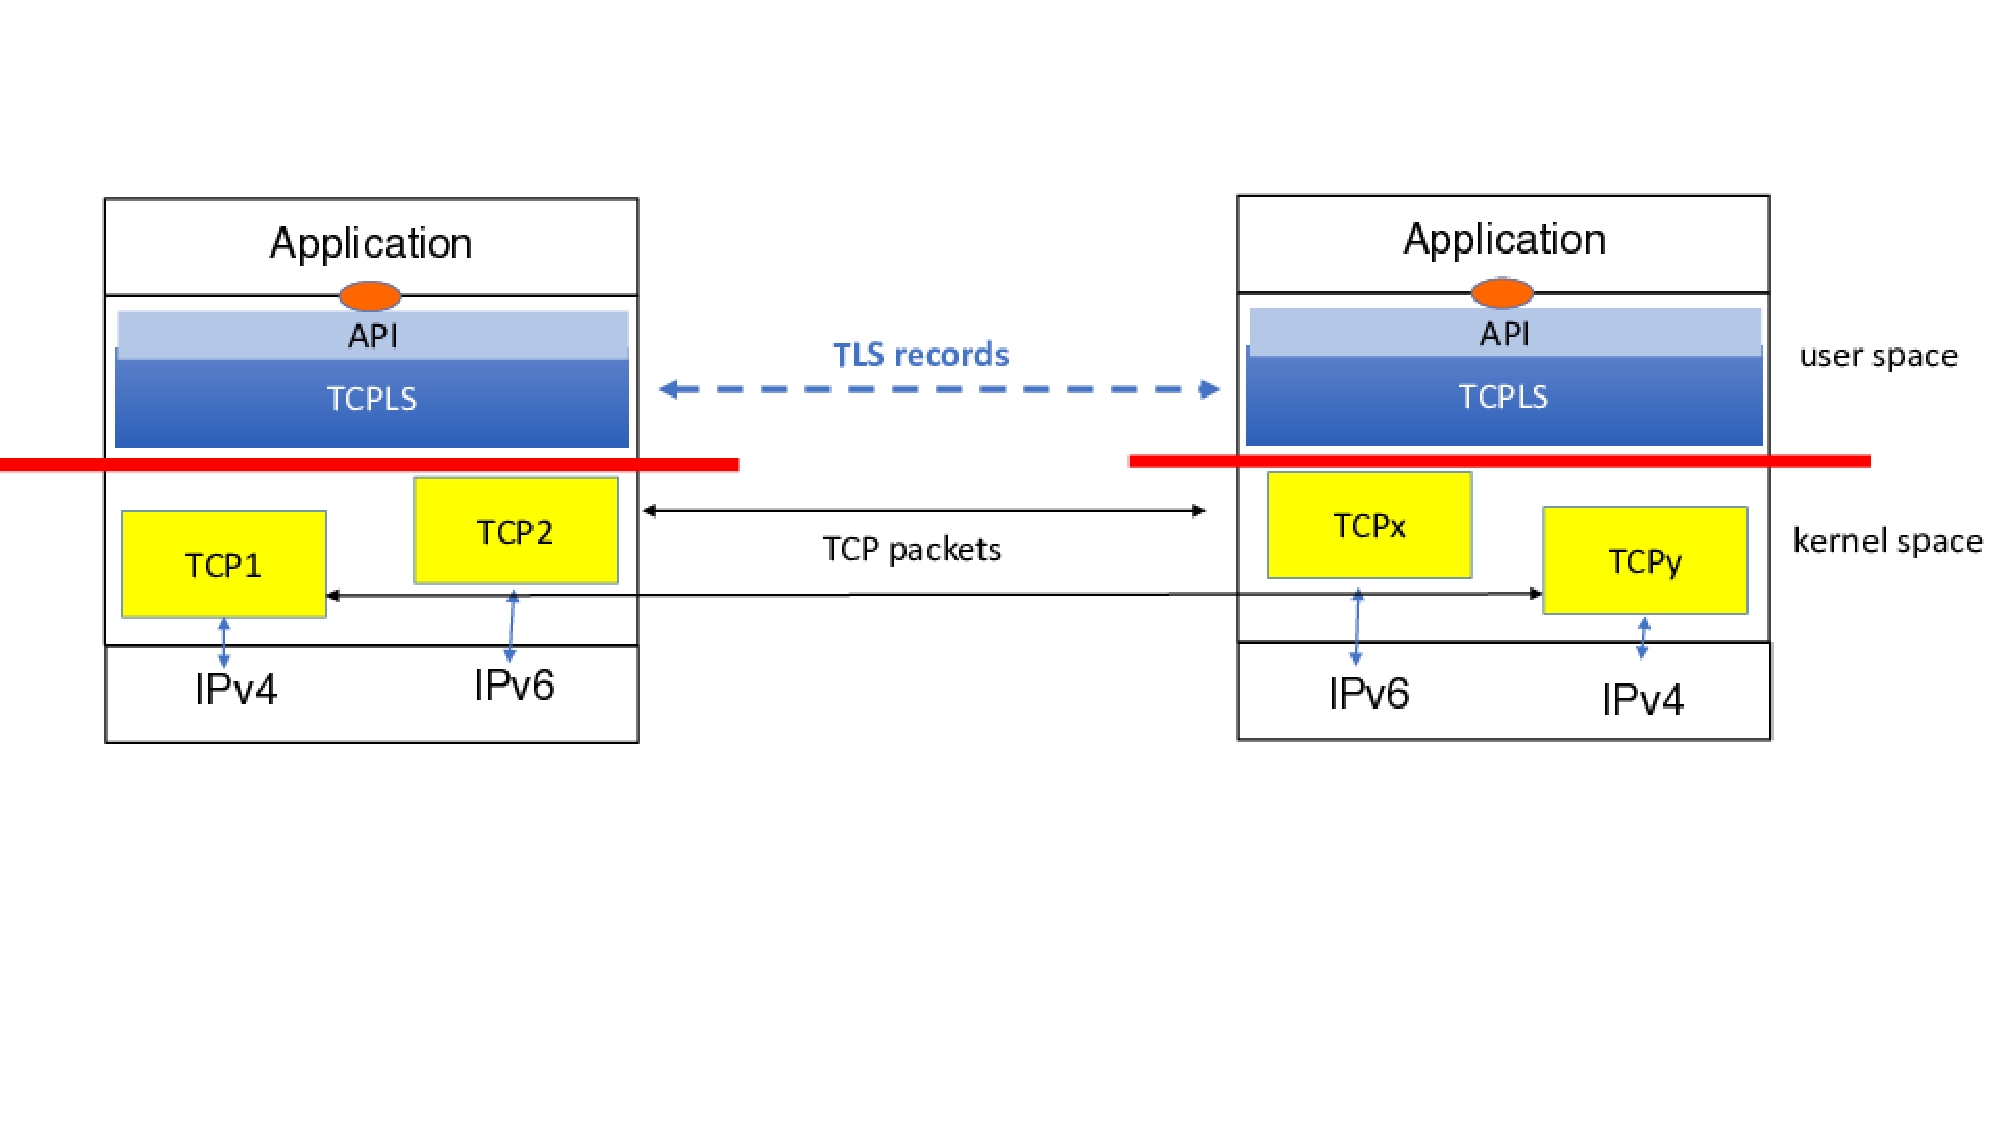
\includegraphics[width=8cm]{figures/tcpls-fig2.pdf}
%  \end{center}
%  \caption{\tcpls in the stack.}
%  \label{fig:arch}
%\end{figure}

 \begin{figure}[!t]
  \begin{center}
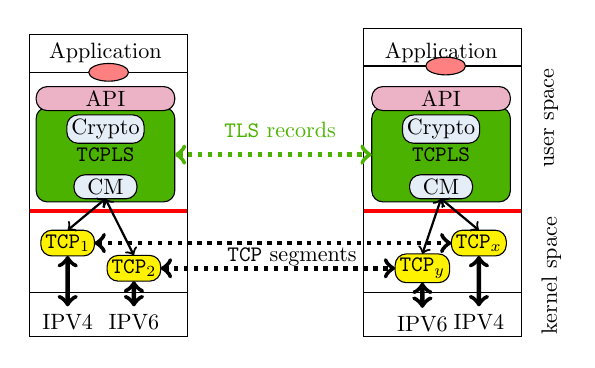
\begin{tikzpicture}[node distance=0 cm,outer sep = 0pt,inner sep = 2pt,  scale=0.80, transform shape]
        \tikzset{application/.style={align=center,minimum height=0.3cm,minimum width=10mm}}
        \tikzset{tcpls/.style={align=center,shape=rectangle,fill=green!70!red!100,minimum height=1.5cm,minimum width=22mm,rounded corners, draw}}
         \tikzset{conman/.style={align=center,shape=rectangle,fill=blue!70!green!10,minimum height=0.15cm,minimum width=10mm,rounded corners, draw}}
        \tikzset{api/.style={align=center,shape=rectangle,fill=purple!30,minimum height=0.15cm,minimum width=22mm,rounded corners,draw}}
        \tikzset{tcp/.style={align=center,shape=rectangle,fill=yellow, minimum height=0.4cm,minimum width=5mm,rounded corners,draw}}
        \tikzset{label/.style={align=center,minimum height=0.5cm,minimum width=5mm}}
        \draw(-3,-0.3) rectangle (-0.5,0.3);
        \draw(-3,-3.8) rectangle (-0.5,0.3);
        \draw [red, ultra thick] (-3,-2.5) -- (-0.5,-2.5);
        \draw(-3,-4.5) rectangle (-0.5,-3.8);
        \draw[fill=red!50] (-1.75,-0.3) ellipse (9pt and 4pt);
        \node[application, xshift=-18mm](application){Application};
        \node[tcpls, below= 6.3mm and 0mm of application](tcpls1){\tcpls};
        \node[api, name=API, below= 3.0mm and 0mm of application, yshift=0mm ](api1){API};
        \node[conman, name=CM, below= 17mm and 0mm of application](cm1){CM};
        \node[conman, name=CM, below= 7.5mm and 0mm of application](crypto){Crypto};
        \node[tcp, below= 4.5mm and 0mm of tcpls1, xshift=-6mm](tcpx1){\texttt{TCP}$_1$};
        \node[tcp, right=5mm and 0mm of tcpx1, yshift=-4mm, xshift=2mm](tcpy1){\texttt{TCP}$_2$};
        \node[label,  below=8mm and 0mm of tcpx1](ip11){IPV4};
        \node[label,  below=4mm and 0mm of tcpy1](ip12){IPV6};


        \draw(2.3,-0.2) rectangle (4.8,0.4);
        \draw(2.3,-3.8) rectangle (4.8,0.4);
        \draw [red, ultra thick] (2.3,-2.5) -- (4.8,-2.5);
        \draw(2.3,-4.5) rectangle (4.8,-3.8);
        \draw[fill=red!50] (3.6,-0.2) ellipse (9pt and 4pt);
        \node[application, right= 0mm and 43mm of application, xshift=-9mm](application2){Application};
        \node[tcpls, name=TCPLS, below= 6.3mm and 0mm of application2](tcpls2){\tcpls};
        \node[api, name=API, below= 3.0mm and 0mm of application2](api2){API};
        \node[conman, name=CM, below= 17mm and 0mm of application2](cm2){CM};
        \node[conman, name=CM, below= 7.5mm and 0mm of application2](crypto){Crypto};
        \node[tcp, below= 4.5mm and 0mm of tcpls2, xshift=6mm](tcpx2){\texttt{TCP}$_x$};
        \node[tcp, left=5mm and 0mm of tcpx2, yshift=-4mm, xshift=-0.3mm](tcpy2){\texttt{TCP}$_y$};
        \node[label,  below=8mm and 0mm of tcpx2](ip21){IPV4};
        \node[label,  below=4mm and 0mm of tcpy2](ip22){IPV6};

        \node[label,  below=8mm and 0mm of application2, xshift=15mm,rotate=90 ](user1){user space};
        \node[label,  below=33mm and 0mm of application2, xshift=15mm, rotate=90 ](user1){kernel space};

        \node[label,  left=of api2, xshift=-5mm, yshift=-5mm, green!70!red!100 ](user1){\tls records};
        \node[label,  left=of ip22, xshift=-5mm, yshift=10.6mm ](user1){\tcp segments};

        \draw[<->,dotted,green!70!red!100,ultra thick] (tcpls1.east) -- node (line) {} (tcpls2.west);
        \draw[<->,dotted, ultra thick] (tcpx1.east) -- node (line) {} (tcpx2.west);
        \draw[<->,dotted, ultra thick] (tcpy1.east) -- node (line) {} (tcpy2.west);
        \draw[<->, ultra thick] (tcpx1.south) -- node (line) {}(ip11.north);
        \draw[<->, ultra thick] (tcpy1.south) -- node (line) {}(ip12.north);
        \draw[<->, ultra thick] (tcpx2.south) -- node (line) {}(ip21.north);
        \draw[<->, ultra thick] (tcpy2.south) -- node (line) {}(ip22.north);
        \draw[<->,   thick] (cm1.south) -- node (line) {}(tcpx1.north);
        \draw[<->,   thick] (cm1.south) -- node (line) {}(tcpy1.north);
        \draw[<->,   thick] (cm2.south) -- node (line) {}(tcpx2.north);
        \draw[<->,   thick] (cm2.south) -- node (line) {}(tcpy2.north);
\end{tikzpicture}
\end{center}
\vspace{-0.5cm}
\caption{\tcpls is implemented as a user space library. The application controls the streams and the underlying \tcp connections through the API. The crypto module manages the security context and the Connetion Manager (CM) controls the utilization of one or more \tcp connections using the kernel stack.}
 \label{fig:arch}
\end{figure}

\subsection{Overview}
%%%%%%%%%%%%%%%%%%%%%%
Today's applications expect more than a simple bytestream from the transport layer. Security is not anymore a requirement for niche application. Applications expect secure transport by default. Similarly, applications are not restricted anymore on using only one network interface. They need to efficiently deal with IPv6 and IPv4 on dual stack hosts and manage the utilization of different network interfaces on mobile devices such as smartphones. \tcpls provides a fast, flexible, and secure transport protocol that is suited for these modern applications. \tcpls is more than the simple addition of the security features of \tls and the reliability features of \tcp. \tcpls leverages \tls 1.3 to negotiate a security context and uses it to send the user data authenticated and encrypted as \tls records. It leverages these records to establish a secure control channel between the client and server. This channel is used to manage the \tcpls session and exchange all control information without any possible middlebox interference. Finally, \tcpls includes a Connection Manager that controls the underlying \tcp connection. The TLS records of a \tcpls session can be transported over different \tcp connections during the session lifetime. This brings several interesting failover and multipath capabilities. Fig.~\ref{fig:arch} illustrates the interactions between two \tcpls hosts. \tcpls can be implemented in userspace within a library like current \tls implementations. It interacts with the \tcp stack that in our prototype resides in the kernel. The crypto module negotiates and manages the security context while the connection manager (CM) manages the utilization of the underlying \tcp connection(s). Closely coupling \tcp and \tls in \tcpls brings opportunities for performance improvement (e.g., avoiding records fragmentation with dynamic receive buffer auto-tuning and/or with dynamic control of the record length), and for connection reliability (e.g., failover).

%\tcpls (illustrated in Fig.~\ref{fig:arch}) offers a cross-layer interface to \tls and \tcp with the motivation to do more than securing the transport layer. Merging the stacks benefits both protocols and the application using this new approach.
%First, \tcp suffers from a lack of extensibility due to size restrictions in its header and due to potential middlebox interferences~\cite{honda2011still}. \tcpls aims to solve \tcp extensibility issue in the long run by offering a secure control channel to exchange \tcp options without suffering from middlebox interferences and size restrictions in \tcp headers.



%\subsection{Overview}

\tcp separates control information and data by placing the control information
in the packet header and the data in the payload. This separation worked well
until middleboxes started to interfere with \tcp~\cite{10.1145/1064413.1064418,
honda2011still}. On a fraction of Internet paths, including e.g., some enterprise and cellular networks, some middleboxes interfere by adding, removing, or changing \tcp options~\cite{wang2011untold,honda2011still,xu2015investigating} and, in some cases, also transparently terminating \tcp connections. These middleboxes have slowed down the evolution of \tcp in recent years. \tcpls also uses the packet header to exchange \tcp control information, but it leverages the extensibility of \tls 1.3 to place control information including some \tcp options inside the \tls handshake messages and new \tls records. Since this information is encrypted and authenticated, the communicating hosts can exchange new control information without encountering middlebox interference. We refer to this exchange of control information as the secure channel between the two hosts.
%We describe several examples of these new types of
%control information in Sec.~\ref{sec:extending} and Sec.~\ref{sec:connmigr}.

A \tcpls session starts with a secure \tls 1.3 handshake ~\cite{rfc8446}. The
client adds a new \tcpls transport parameter in its \textsc{ClientHello} message. A \tcpls server replies with a \textsc{ServerHello} message that negotiates the security keys and may include additional \tcpls information as
\textsc{EncryptedExtensions}. After this secure handshake, the client and the
server have a shared security context.

As \sctp~\cite{rfc4960} or \quic~\cite{draft-ietf-quic-transport}, \tcpls
supports one or more streams over a single \tcpls session. An application
can open, attach, and close streams to an existing \tcpls session. Each
stream is an independent cryptographic context derived from the \tcpls
security context. The \tcpls streams can carry application data
or control information.

%They must be attached to a \textit{Connected} \tcp bytestream exported as a \texttt{transportid} to the application. To manipulate streams, \tcpls offers an API to open, attach
%and close streams to any available \texttt{transportid} in the \textit{Connected} state, while offering the Stream as the only bytestream abstraction to the upper layer. Streams can only be attached to one \texttt{transportid}, but they can be moved, several streams can be attached to a given \texttt{transportid}, and multiple streams can be attached to multiple \texttt{transportid}s.

To attach a new stream, a host simply sends the \texttt{STREAM\_ATTACH} message as a special \tls record over the secure channel. Since each stream is an independent cryptographic context, the recipient can immediately start to decrypt and extract data from the new stream. No round-trip is wasted to attach a new stream.

%\tcpls can attach streams using the Secure Control Channel and send TLS records
%within them in a zero-rtt fashion. That is, when the peer receives a
%\texttt{STREAM\_ATTACH} message in the control channel, it has everything needed
%to securly derive the right cryptographic context to process the TLS record
%encryted within this stream. No round-trips are needed to attach a new stream.
%Most of records encrypted with a Stream's context contain application data
%transmitted by the client or the server. However, streams can also carry control
%records.

%The control channel between the client and the server
%enables \tcpls to define a new bytestream abstraction and support many new
%features while benefitting from the current kernel and network optimization for
%\tcp performance.

%Applications such as HTTP/2 support multiple streams mapped to a single \tcp
%connection. However, there are situations, e.g., to prevent head-of-line
%blocking, where different streams should be mapped over other underlying \tcp
%connections. With \tcpls, the client and the server can establish different
%datastreams over a single \tcpls session, preventing \tcp's HOL. Thus, a
%\tcpls session can be composed of one or more \tcp connections similarly as a
%\mptcp connection gathers subflows.

\tcpls' Connection Manager controls the utilization of the underlying \tcp connections. It can open, close, or reestablish failed \tcp connections. Each of
the connections that composes a \tcpls session is identified by a \emph{transport identifier}. By default, the data from a stream can be sent over any of the underlying \tcp connections. The applications that require finer control over the utilization of the underlying \tcp connections can use the \tcpls API to map a stream on a specific underlying connection. In this case, all the data of this stream is exchanged over this specific connection. By placing two streams on different connections, an application can prevent Head-Of-Line (HOL) blocking among these streams.

\tcpls also supports failover and multipath. To support these features, it
must be possible to send data from a given stream over different \tcp connections. In this case, the \tcp level sequence numbers and acknowledgements are not sufficient anymore to enable the receiver to reorder the data. When this feature
is enabled, \tcpls its own sequence numbers and acknowledgements that are exchanged as new \tls records over the secure control channel.
Thanks to these \tcpls acknowledegments, a \tcpls session can survive to
the failure of the underlying \tcp connection by reestablishing a new
\tcp connection to continue the data transfer and replay the lost records.

A \tcp connection ends with the exchange of \fin or \rst packets. However, some
middleboxes force the termination of \tcp connections by sending \rst
packets~\cite{rfc3360,weaver2009detecting}. \tcpls can preserve established
connections by automatically restarting the underlying \tcp connection upon
reception of a spurious reset. \tcpls defines the connection termination at the
stream level: a \tcpls session is closed once the last stream attached to a
\tcp connection is securely closed.

That is, \tcpls' Secure Control Channel provides a flexible abstraction
to the upper layer that supports various new features such as
Streams, connection reliability, different secure multipath modes, secure
connection closing, encrypted \tcp options and leverages \tcp's performance and \tls's state of deployment.

%Todo explain that the transport abstraction level failed to offera versatile
%usage
%of the transport layer, and explain how a session layer can repair the
%abstraction
%Besides, with our design of \tcp extensibility
%within \texttt{\tcpLS}, applications would be able to tune \tcp on a connection basis,
%using existing options or any future option without middlebox interferences. As
%a matter of example, our \texttt{\tcpLS} implementation supports several
%\tcp options that can difficulty live at the \tcp layer
%(e.g., Joining a Multipath connection, injecting eBPF bytecode to the kernel's
%peer to tune \tcp). With \texttt{TCPLS}, we show how to solve several of these
%existing problem.

%Finally, \texttt{\tcpLS}'s control channel is expected to offer extensibility
%without middlebox interference and with protocol message indistinguishability
%from the network to avoid fingerprinting of the client stack. Our objective is
%to design a versatile \tcp extensibility mechanism that would allow to set
%options, exchange eBPF bytecode~\cite{de2019pluginizing} to tune the peer's kernel and implement new
%session behaviours.

% !TEX root = ./paper.tex

\subsection{\tcpls Transport Services}
\label{sec:transport-services}

%\todo{parler de secure control channel ? (mp): Pour moi non, c'est une vue de
%l'esprit, ça équivaut a dire qu'on peut utiliser des nouveaux records tls}

By leveraging \tcpls records and extensions, we can design new modern transport
services atop the combination of \tcp and \tls. In this subsection, we answer 
our second research question {\small\textit{RQ2}} by presenting three transport 
services: stream multiplexing (Section~\ref{sec:datastreams}), connection 
migration (Section~\ref{sec:multipath}), and bandwidth aggregation 
(Section~\ref{sec:multipath}). We leverage the \tcpls records
to multiplex concurrent encrypted bytestreams. By extending the \tls handshake, \tcpls allows joining several \tcp connections to a single \tcpls session to support
connection migration and %multipath capabilities, mitigating Head-of-Line
%blocking and enabling
bandwidth aggregation.
%aggregation and Head-of-Line blocking resilience.

\subsubsection{Stream Multiplexing}\label{sec:datastreams}
%%%%%%%%%%%%%%%%%%%%%%%%%%%%%%%%%

\begin{figure}[!t]
	\centering
	\begin{bytefield}[bitheight=\widthof{aw}]{32}
		\bitbox[]{1}{\small N} & \bitbox[]{9}{} & \bitbox[]{3}{\small N-32} &
		& \bitbox[]{7}{} &
		\bitbox[]{1}{\small 64} & \bitbox[]{9}{} & \bitbox[]{3}{\small 0} \\
		\bitbox{32}{TLS 1.3 AEAD Initial Vector}  \\
		\bitbox[]{12}{+} & \bitbox[]{8}{} & \bitbox[]{12}{$\oplus$} \\
		\bitbox{12}{\tcpls Stream ID} & \bitbox[]{8}{} & \bitbox{12}{Record sequence}
	\end{bytefield}
	\caption{The AEAD IV of \tcpls Streams is derived from \tls 1.3}
	\label{fig:aead-iv}
\end{figure}

Stream Multiplexing is a transport service that has been part of recent
protocols such as \sctp~\cite{rfc4960}, \quic~\cite{rfc9000} and HTTP/2.0
\cite{rfc7540}. The latter also proposes multiplexing with an independent
framing system atop the \tls-encrypted \tcp bytestream. In \tcpls, we choose to
implement multiplexing with \tcpls records. We dedicate a \tcpls record type to
\tcpls stream data. Each stream has a separate cryptographic context allowing
concurrent encryption and decryption of data within the same session.  A \tcpls
stream consists of a sequence of \tcpls stream data records encrypted with their
cryptographic contexts. Each stream is attached to one \tcp connection.

One simple way to provide separate cryptographic contexts is to use multiple
application-level keys. But this is known to degrade the security properties
proportionally to the number of additional keys~\cite{chatterjee2011another}. To
overcome this, we propose an Initial Vector (IV) derivation technique that
enables independent encryption/decryption to each stream without the security
degradation.

Figure~\ref{fig:aead-iv} illustrates how the AEAD IV is computed for a given
\tcpls record of a \tcpls stream. First the left-most bits of the IV derived
from the \tls handshake are summed with the 32-bit \tcpls Stream ID. Then the
right-most bits are XORed with the stream 64-bit record sequence number. Each
\tcpls stream has a separate record sequence number space. This combination of
IV manipulation guarantees that the resulting IV is unique for each record of
all \tcpls streams as long as the Stream ID is unique and no sequence number is
used twice in a given stream. The Stream ID space is split between the client
and the server. Stream ID 0 is equivalent to the cryptographic context directly
derived from the handshake.
%\todo{Il faut expliquer comment les stream id sont choisis pour garantir
%l'unicité}

To avoid possible middleboxes interference, in addition to the record sequence
number, the \tcpls Stream ID is kept implicit as well. When an endpoint receives
a \tcpls record, we leverage the AEAD cipher to check the authentication tag
repeatedly until the correct \tcpls Stream ID is found. An optimized
implementation would not involve a complete decryption as all TLS 1.3 AEAD
ciphers use an Encrypt-then-MAC construct~\cite{rfc7366, rfc8446}, and the tag
verification, especially on AES-GCM is computationnaly light.
%\todo{citer rfc7366 ? ou les références de ce rfc ?}

From a security standpoint, each failed decryption is considered as a forgery
attempt. However, the limits on confidentiality and integrity for AEAD ciphers
are large before a successful forgery may be considered with non-negligible
probability~\cite{luykx2015limits, aeadlimits}. For example, in the case of
ChaCha20 + Poly1305, an adversary making $2^{60}$ forgery attempts succeeds with
probability $2^{-33}$.
%\todo{Should we mention that one stream cannot be used on two connections at the same time?}

%The classical solution to support streams in a transport protocol is to assign
%an identifier to each stream and send the data from stream $x$ as a tuple
%$x,seq,data$ where $seq$ is a sequence number. This is the solution chosen by
%\sctp~\cite{rfc4960} and \quic~\cite{draft-ietf-quic-transport}. \tcpls relies
%on cryptographic properties to support several streams.

%\paragraph*{Cryptographic Details and Tricks} In \tcpls, each stream has its own
%cryptographic context. All streams use the same key but derive a specific
%Initial Vector (IV - also called cryptographic nonce) such that nonce-misuse
%cannot happen. Furthermore, \tcpls derives the IV such that the record sequence
%numbers can securely start at $0$ within each stream.
%
%\tcpls uses only one application-level key for $N$ streams, for each direction.
%We selected this approach to avoid security degradation with the usage of
%multiple keys (by a factor $k$ with $k$ keys)~\cite{chatterjee2011another}.

%To enable all stream sequence numbers to start at 0, we rely on some properties
%of the Authenticated Encryption with Associated Data (AEAD) schemes used by \tls
%1.3. To preserve AEAD security, the AEAD nonce used by \tcpls must be of unique
%use when encrypting and decrypting a record. The initial nonce must also be
%unpredictable for an adversary observing the handshake. \tcpls derives it from
%the \tls handshake session secret in a similar fashion to the \tls
%keys~\cite{rfc8446}. The nonce size ranges from $96$ bits to $128$ bits
%depending on the underlying cipher used. In all cases, for a nonce of size $N$
%bits, \tls computes the cryptographic nonce by concatenating the $N-64$ leftmost
%bits with the 64 lower bits XORed with the record's implicit sequence number
%encoded in 64 bits. XORing the lower 64 bits provides more unpredictability to
%the nonce when the same plaintext is encrypted multiple times with the same
%key~\cite{bellare2016multi,hoang2018multi}. This design implies that we give to
%the underlying cipher the 32 upper bits untouched. The resulting value is then
%concatenated with an internal counter in GCM and used as the blocksize-bits (128
%or 256 bits) stream's counter.
%We observe that the leftmost N-64 bits are available to encode a unique stream number. By
%encoding such a unique number in this part of the cryptographic nonce, we enable
%each stream to start its sequence number at 0 while encrypting its records with
%the same key. This observation means that we can create independent
%cryptographic contexts based on a cryptographic nonce's tweak. This implies
%that stream records can be encrypted and decrypted independently of each other,
%with the same key value. This technique maintains AEAD's core assumption
%(uniqueness of nonce), which means that state of art AEAD's security proof
%starting from that assumption applies to our
%design~\cite{chatterjee2011another} and guarantees the security of our scheme.

%\paragraph*{Carrying Multiple Streams over the Same Transport}
%(mp): TODO Multicore decryption could be listed as an improvement
%Thanks to those separate cryptographic contexts, \tcpls can perform concurrent
%encryption and decryption between streams while maintaining decryption
%correctness and security, and potentially also use this capability to process
%different streams over different CPU cores.
%Finally, when different streams are carried
%over the same \tcp connection, \tcpls does not explicitely know which stream
%a received record belongs to. To retrieve this information,
%we also
%leverage the AEAD cipher and check the incoming record's authentication tag
%until we find the stream that properly verifies this tag. This operation is
%lightweight: it does not require full decryption of the record because the AEAD
%ciphers used by \tls 1.3 do Encrypt then MAC (and MAC then Decrypt).
%Looking for the right stream that succeeds the tag verification needs to be
%performed once each time the application writes to another stream over the same
%\tcp connection.
%
%Note that, security-wise, each failed decryption is considered a
%forgery attempt. However, we have large limits on the confidentiality and
%integrity with all AEAD ciphers~\cite{luykx2015limits, aeadlimits} before a
%successful forgery may be considered as a non-negligible probability. For
%example, in the case of ChaCha20 + Poly1305, an adversary making $2^{60}$ forgery
%attempts succeeds with probability $2^{-33}$.


\subsubsection{Connection Migration}\label{sec:multipath}

\tcpls allows joining several \tcp connections to an existing \tcpls session.
We leverage this mechanism to implement new transport services such as connection migration. Compared to the subflow joining mechanism of
\mptcp~\cite{raiciu2012hard,hesmans2015smapp,hesmans2016enhanced}, our design is
more secure. Indeed, \mptcp supports additional subflows by initially exchanging
short keys inside cleartext \tcp \texttt{Options} during the \tcp handshake~\cite{rfc6824, rfc8684}. These keys are then used to authenticate the association of subflows. An attacker having observed the key exchange during the \tcp handshake can associate subflows to an existing \mptcp connection~\cite{rfc6181}.

\begin{figure}[!t]
	\centering
	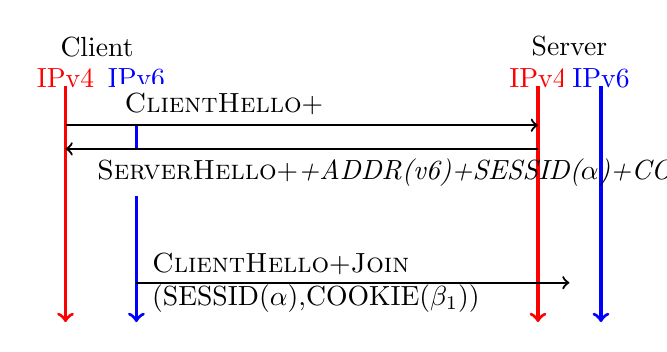
\begin{tikzpicture}
		\colorlet{lightgray}{black!20}
		\tikzstyle{arrow} = [thick,->,>=stealth]
		\tikzset{state/.style={rectangle, dashed, draw, fill=white} }
		\node[black, fill=white] at (0,10) {Client};
		\node[black, fill=white] at (6,10) {Server};
		\node[red, fill=white] at (5.6,9.6) {IPv4};
		\node[blue, fill=white] at (6.4,9.6) {IPv6};
		\node[red, fill=white] at (-0.4,9.6) {IPv4};
		\node[blue, fill=white] at (0.5,9.6) {IPv6};
		\draw[red, very thick,->] (-0.4,9.5) -- (-0.4,6.5);
		\draw[blue, very thick,->] (0.5,9.5) -- (0.5,6.5);
		\draw[red, very thick,->] (5.6,9.5) -- (5.6,6.5);
		\draw[blue, very thick,->] (6.4,9.5) -- (6.4,6.5);
		\draw[black, thick, ->] (-0.4,9) -- (5.6,9) node [midway, fill=white, above,
		text width=4.5cm] {\textsc{ClientHello}+\hello};
		\draw[black, thick, <-] (-0.4,8.7) -- (5.6,8.7) node [pos=0.5, fill=white, below, text width=5.2cm] {\textsc{ServerHello}+\emph{\hello+ADDR(v6)+SESSID($\alpha$)+COOKIE($\beta_1,\beta_2$)}};
		\draw[black, thick, ->] (0.5,7) -- (6.0,7) node [pos=0.4, %fill=white, above,
		text width=4cm] {\textsc{ClientHello}+\join(SESSID($\alpha$),COOKIE($\beta_1$))};
	\end{tikzpicture}
	\caption{\tcpls supports joining additional \tcp
		connections to a \tcpls session. The $SESSID$ and $COOKIE$ in the \textmd{\textsc{ServerHello}} are encrypted with the
		handshake key.}
	\label{fig:join-example}
\end{figure}

\textbf{Joining \tcp connections}. \tcpls leverages \tls
extensions to solve this problem in a more secure manner. 
Figure~\ref{fig:join-example} illustrates the \tls and \tcpls messages 
exchanged when a client connects to a server over IPv4 and later joins another 
connection over IPv6.
First, the client sends a \textsc{ClientHello} containing a \hello. The server 
replies with a \textsc{ServerHello} containing three encrypted extensions. 
First, the server announces its IPv6 address ($ADDR(v6)$). Second, it 
associates one identifier $\alpha$ to the \tcpls session 
(\emph{SESSID($\alpha$)}).
%It uniquely identifies the \tcpls session on the server.
Third, the server provides a list of \tcpls session cookies $\beta_1,\beta_2$ in the \emph{COOKIE} extension. Each of these session cookies enables the client
to join one additional \tcp connection to the \tcpls session. Thus by 
sending $n$ cookies over a session, the server restricts the client to 
join up to $n$ \tcp connections. This prevents resource exhaustion attacks
that are difficult to counter with \mptcp. The server can later send additional
cookies and update its list of addresses.

To join a new \tcp connection to the \tcpls session, for instance over IPv6, the
client sends a \textsc{ClientHello} message containing the session identifier
(SESSID($\alpha$) in Figure~\ref{fig:join-example}) and one of the cookies
provided by the server (COOKIE($\beta_1$) in Figure~\ref{fig:join-example}). The
server uses the session identifier $\alpha$ to find the corresponding \tcpls
session and checks the validity of the cookie. If the \tcpls session and cookie
are valid, the \tcp connection is joined to the \tcpls session. The session
identifier plays the same role as the \mptcp token, but is sent encrypted. The
cookie provides stronger protection than \mptcp's HMAC with security keys
exchanged in cleartext. The \tcpls cookies are sent encrypted by the server and 
can only be used once by the client.
%(i.e.,
%when the server receives a valid cookie, it accepts the connection, attaches it
%to the right \tcpls session, and discards the cookie).


%\tcpls includes a Connection Manager (CM) that controls the underlying \tcp
%connections.
%The CM is fully configurable and exposed to applications through the \tcpls API.
%\tcpls enables the client or the server to associate new \tcp connections to an
%existing \tcpls session. This is similar to \mptcp's path
%managers~\cite{raiciu2012hard,hesmans2015smapp,hesmans2016enhanced},
%but with some differences. First, \tcpls does not suffer from the same
%security limitations as \mptcp. Second, \tcpls supports several multipathing
%modes, including connection failover, bandwidth aggregation and non-aggregated
%multiple paths.

%\paragraph*{1) Better Security Than \mptcp} A \mptcp connection gathers several
%underlying connections called subflows. To ``secure'' the attachment of
%additional subflows, \mptcp hosts exchange short keys in plaintext inside \tcp
%options during the \tcp handshake~\cite{rfc6824, rfc8684}. These keys are then
%used later to authenticate the attachment of subflows. An
%attacker that has observed the initial handshake can attach any subflow to an
%existing \mptcp connection~\cite{rfc6181}. \tcpls leverages its secure channel
%to solves this \texttt{``connection join''} problem in a more secure
%manner. Consider a client connecting to a dual-stack server
%(Figure~\ref{fig:join-example} depicts the \tls messages exchanged in such a
%scenario). The client sends a \textsc{ClientHello} containing the \tls
%extension to negotiate \tcpls. The server replies with a \textsc{ServerHello}
%with three types of encrypted extensions. First, the server announces its IPv4
%and IPv6 addresses. Second, it associates one identifier to the \tcpls session
%(SESSID($\alpha$) in Figure~\ref{fig:join-example}). It uniquely
%identifies the \tcpls session on the server. Third, the server provides a list
%of \tcpls session cookies (COOKIE($\beta_1,\beta_2$) on
%Figure~\ref{fig:join-example}). Each of these session cookies enables the 
%client
%to attach one additional \tcp connection to the \tcpls session. By sending $n$
%cookies, the server indicates that it currently accepts the attachment of only
%$n$ \tcp connections to this session. This prevents resource exhaustion attacks
%that are difficult to counter with \mptcp. The server can send additional
%cookies later and update its list of addresses.
%
%To attach a new connection, e.g., using the server's IPv6 address, the client
%sends a \textsc{ClientHello} message containing the session identifier
%(SESSID($\alpha$) on Figure~\ref{fig:join-example}) and one of the server's
%cookies (COOKIE($\beta_1$) on Figure~\ref{fig:join-example}). The server checks
%the validity of the cookie and then uses the session identifier to attach the
%new \tcp connection to the right \tcpls session. The session identifier and
%cookie play that same role as \mptcp's token. From a security viewpoint, \tcpls'
%session cookie is longer than \mptcp's token. Furthermore, it is sent encrypted
%in the initial \textsc{ServerHello} message, and can only be used once (i.e.,
%when the server receives a valid cookie, it accepts the connection, attaches it
%to the right \tcpls session, and discards the cookie).

\begin{figure}[!t]
	\begin{center}
		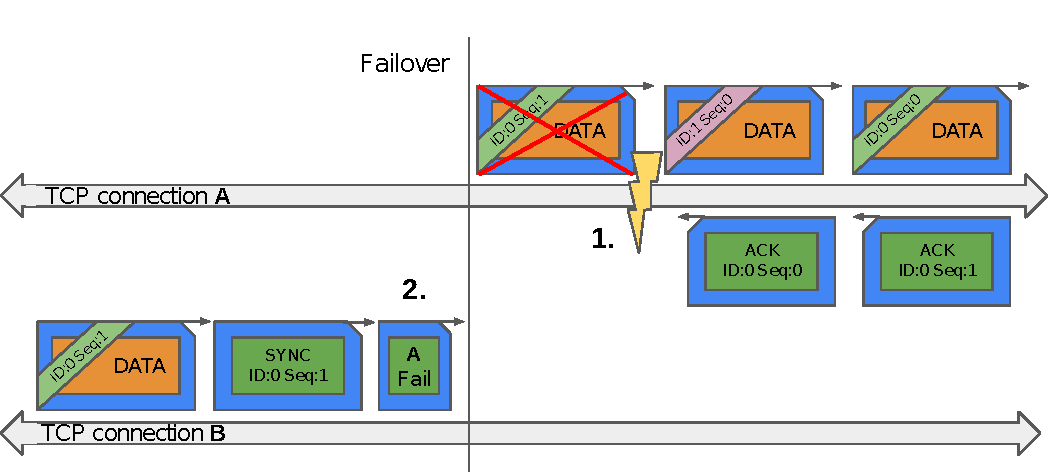
\includegraphics[width=\columnwidth]{figures/tcpls_failover}
	\end{center}
	\caption{Failover resynchronises and retransmits lost \tcpls records 
	from a failed \tcp connection to an other.}
	\label{fig:failover}
\end{figure}

\textbf{Failover}.
When a \tcp connection fails, e.g. due to middleboxes or network outages, 
\tcpls leverages its joining mechanism to recover 
the session over another \tcp connection. Figure~\ref{fig:failover} illustrates 
how \tcpls reacts to such events during a transfer with two \tcpls streams.
To achieve such a \emph{break-before-make}, 
\tcpls sends acknowledgments for the received records of each stream, allowing
the sender to remove them from its sending buffer.
%Upon reception of Stream-level acknowledgments, the sender can
%manage its sending buffer and remove acknowledged encrypted records. 
When the \tcp connection fails, the sender switches to the other one and 
explicitly notifies the failure to the receiver. The sender then synchronizes 
the transmission sequence using a dedicated \tcpls record type (i.e. SYNC in 
Figure~\ref{fig:failover}) and retransmits the 
unacknowledged stream data records (i.e. the second record of stream 0 in 
Figure~\ref{fig:failover}). 
Explicit synchronization %is required as the \tcpls stream sequence number is 
%implicit and thus 
prevents a lost acknowledgment from desynchronizing the endpoints. 
Thanks to the per-stream cryptographic context, the ciphertext of lost stream 
data records can be retransmitted as is.

%Furthermore,
%the unacknowledged data records sent over the failed \tcp connection are
%transmitted again over a functional one. To resynchronize the session (i.e., 
%the
%implicit encryption/decryption sequence numbers), the
%failover protocol makes the client sends the sequence number of the first 
%record
%within its sending buffer, an $id$ to specify the failed \tcp connection and
%the Stream ID of the stream being moved. This information is encrypted with
%the default context and sent within the new \tcp connection. Receiving this 
%protocol message, the server now knows
%the sequence number to decrypt some record arriving next on the connection that
%read the failover message. Either the server already processed that record, 
%and can safely
%ignore it and increase the sequence number, or the server did not yet seen that
%record, and can decrypt and process it. The same protocol message and 
%operations
%then goes from the server to the client, and the stream is then resyncronized
%over a new \tcp connection. No messages are required to be encrypted twice.
%\tcpls' Failover mode is optional. Both peers need to activate it or
%negotiate the feature throught the Secure Control Channel.
We present in Section~\ref{sec:perf} measurements quantifying the
performance impact of adding \tcpls record-level acknowledgments. We also
present in Section~\ref{sec:eval_failover} an analysis of recovery speeds during
different type of outages.
%We also give a
%trace example involving a file transfer and the failover protocol in
%Appendix~\ref{app:failover}.
%\todo{Let see if we can bring it back in the text later}

\textbf{Application Connection Migration}. \tcpls also enables the
application to trigger a connection migration, for instance based on application-level metrics qualifying its experience over the current path.
%expected to be used
%over
%healthy networks. %and leveraging a transient usage of bandwidth aggregation.
%(mp): I would leave this aside for now, until we explain application streams.
%The decision to migrate from a healthy network to another one is a
%application one.
%(mp): Yet the following meta-info are not described, and again implementation
%-> section
%4
\tcpls enables the exchange of meta-information to help this
decision.
%The TCPLS protocol and implementation's job is to make it quite simple by
%supporting the exchange of interface's related meta-information to help the
%decision
%making and by offering a simple API.
%Essentially, it means that \tcpls provides a simple API that enables an
%application to migrate when it wishes to do so (e.g.,
For instance, an interactive application running on a smartphone could migrate 
from
LTE to Wi-Fi when it senses an increase in delays due to bufferbloat for a
given period of time, or when a mobile client detects its home Wi-Fi and the
user's preference is to move its traffic to the Wi-Fi if detected.
%when the Wi-Fi appears healthy,
%The semantic of
%the application-level connection migration is built from attaching and closing
%streams in the multipath bandwidth aggregation mode.
%The client that wishes to
%carry such a migration first creates a new \tcp connection and joins the \tcpls
%session over this connection.
To achieve it, the client moves all its \tcpls streams to another \tcp
connection.
%(mp): avoid introducing concepts we define later rather than earlier
%can essentially use Stream Streering, i.e., the client
%\textit{composes} with independent
%features offered by \tcpls.
%(mp) -> section 4
%In a client/server implementation using \tcpls, the
%following protocol composition is realised with only 4 API calls (4 lines of
%code).
First, it creates a new \tcp connection and joins it to the
\tcpls
session. Then, %it steers the \tcpls stream abstraction,
it attaches new streams to the new
connection
%using the stream opening protocol
and removes the old ones from the underperforming connection, effectively moving
the application traffic to the new connection.
%(mp): Lets talk of that in the following section rather
%This stream steering
%mechanism may temporally takes advantage of bandwidth aggregation during the
%fraction of seconds required to open the second stream and close the first one.
%These properties are latter demonstrated in Section~\ref{sec:app-migration}.

%by sending one \textsc{Stream\_Attach} message per stream that needs
%to be migrated. At that moment, the client and the server have potentially
%multiple streams opened over the two network paths and can temporally aggregate
%the bandwidth offered by both paths. Then, after having attached
%all its streams to the new path, the migrating host sends a
%\textsc{Stream\_Close} message over the old \tcp connection for all old streams.
%At this point, the migrating host cannot send new stream data anymore over the
%old connection. Once the remote host has received a \textsc{Stream\_Close}
%message over the old \tcp connection, it knows that the connection is not
%available anymore\todo{?}, and can switch to the other connections. It first sends a
%\textsc{Stream\_Close\_Ack} message for each received \textsc{Stream\_Close}.
%The migrating host can close the old connection upon reception of the last
%\textsc{Stream\_Close\_Ack}, indicating that no more data would be received over
%this connection. Note that these messages are \tls records and are thus sent
%securely and reliably.% by the underlying \tcp connection.

This second type of migration does not require application-level
acknowledgments, but it cannot survive from one of the
underlying connections' failure. During such a migration, data may be sent over
two connections, which brings us to explain how multipath is designed.

\subsubsection{Multipath capabilities}

Like \mptcp, \tcpls allows an application to control different \tcp connections
that are used to exchange data. \mptcp was designed to be a drop-in replacement
for \tcp. A regular application that uses the socket API can use \mptcp without
any modification. \mptcp uses a path manager to control the underlying \tcp
connections. Several path managers were proposed in the Linux kernel
implementation \cite{TODO}.\todo{ref} However, few advanced applications have taken
advantage of these advanced path managers. Apple's \mptcp stack was tuned for
specific applications. For example, the Siri voice recognition application can
use both cellular and Wi-Fi to optimize performance. Apple Music mainly uses 
\mptcp to perform seamless handovers. As applications have very different 
requirements, \tcpls
exposes the underlying \tcp connections to the application through its API. The
applications use this API to implement their own policy to manage the
underlying \tcp connections.

%(mp): It's already part of related work actually
%When several networks paths are used in a transport
%connection, the congestion controller of each path should be coupled to control
%the overall aggressiveness of the connection. This problem has been solved in a
%generic way for MPTCP~\cite{rfc6356}, and the same solution could be applied to
%\tcpls. eBPF could be leveraged to access and modify the congestion controller
%state. We leave this engineering effort as future work.

\textbf{Stream Steering}. \tcpls enables the application to combine
multiplexing with the ability to join
several \tcp connections to a \tcpls session. This allows the application to
steer \tcpls
streams over the different \tcp connections. While Failover moves
\tcpls streams from one connection to another when a \tcp connection fails, stream
steering allows the application to distribute at any time the streams over the
different
\tcp connections of a \tcpls session. We already discussed a very simple use of
stream steering when performing Application Connection Migration %, which plays
%with opening, attaching and closing \tcpls stream protocols 
to move application data to a new connection.

%Like \mptcp \cite{raiciu2012hard,rfc6824} or Multipath QUIC
%\cite{de2017multipath,draft-liu-multipath-quic-02}, \tcpls supports an
%aggregation mode that maps data over two or more \tcp connections. On multihomed
%hosts, this can increase the total throughput of a \tcpls session by spreading
%the data over different network interfaces. In this case, one or more data
%streams are mapped to two or more underlying \tcp connections and \tcpls
%schedules different records over different connections.

Applications assign \tcpls streams to \tcp connections through the \tcpls
API.
%The choice of assigning to the \tcpls streams to the \tcp connections is left
%to the application through the \tcpls API.
An interactive game could use different streams for chat messages and player's
commands.  Also, an HTTP server could choose
the \tcp connection for the stream of each response based on the content type of
the response. Latency-critical objects could be sent over
low-latency connections. By sending each application-level object in a separate
stream, the application can benefit from multiple network paths while
maintaining the ability to process each stream in a zero-copy manner, and
with no head-of-line blocking.
\tcpls enables the application to choose which streams are protected from
Head-of-Line blocking by placing them on separate \tcp connections.
%Applications objects that depend on others can cope with occasional
%Head-of-Line blocking.

%\todo{Choix du HoL, ça coute des connexions mais pas forcément nécessaire en
%	fonction de l'app.}

%\todo{OB: paragraphe ci-dessous pas clair. (mp): C'est m-à-j}
%\todo{Multipath congestion control appliqué a TCPLS, eBPF, pas trivial}

\textbf{Coupling streams for aggregated bandwidth}. 
%Recall that each stream isbattached to only one \tcp connection. 
Applications that benefit
from the aggregated bandwidth of several network paths when transmitting a
single application object can use \tcpls \textit{coupled streams}. Coupled
streams send data alongside a sequence number located at the end of
the record. The sender can schedule \tcpls records of an application
object over these streams and benefit from their aggregated bandwidth by 
sending data over the two streams using a strategy that fits the application 
usage. The receiving application reads the application object in order, as 
\tcpls handles the reordering of coupled streams decrypted records.
%That is, with coupled streams, \tcpls offers
%to the application an explicit interface to the sender, and an agnostic
%interface to the receiver
%This provides a level of service similar to MPTCP and MPQUIC.

Dozens of packet schedulers were proposed for \mptcp. The default one is the
RTT-based scheduler that favors the subflow with the lowest RTT
~\cite{paasch2014experimental}. Other schedulers include the redundant
scheduler
that sends data over both subflows~\cite{frommgen2016remp}, schedulers that
help to minimize reordering on the receiver side~
\cite{lim2017ecf,hurtig2018low}, schedulers specialized for mobile
applications~\cite{de2018tuning}, \ldots
The most flexible approach remains the application-defined Multipath TCP
scheduler~\cite{frommgen2017programming}, but this solution has never been
integrated in \mptcp implementations.

\tcpls takes a different viewpoint. It exposes the underlying \tcp connections
and the sender side \tcpls record scheduler to the application. This enables
the application to actively decide the \tcp connection that it will use to send
each record. A remote terminal application running over \tcpls could send the
screen updates over a high bandwidth but high latency connection and the
keyboard input over the lower latency one.
%(mp): On ne peut pas il me semble
Using socket options such as
\texttt{tcp\_info}, an application can retrieve useful statistics about the
performance of the underlying \tcp connections (e.g. RTT, congestion window,
\ldots). %If required, it is also possible to
A more advanced application could also define \tcpls records to actively
probe a connection, e.g. with an echo/request record to actively measure
delays, or retrieve information from the remote host, e.g. by retrieving the
remote host's \texttt{tcp\_info} structure.

Coupled streams can be used when performing Application Connection
Migration to smoothly transition from one network path to another without
impacting the application goodput.

%In this subsection, we also present how streams can be coupled to aggregate
%the
%bandwidth of several \tcp connections.
%This provides various types of services,
%such as easily performing active migration as discussed in the previous
%Section~\ref{sec:multipath}. Bandwidth aggregation can also be activated. It is
%also possible not to activate aggregation and reording to obtain
%independent streams carrying independent application-level objects, which would
%prevent head-of-line blocking similarly to \quic.


%In addition, \tcpls allows the application to attach its streams to the
%underlying \tcp connections in a non-aggrega-ted bandwidth mode. This is a
%choice left to the application using the API. It has several advantages and
%drawbacks compared to the aggregation mode. For example, the aggregation mode is
%simple to use and can potentially saturate the available network paths but can
%lead to Head-Of-Line (HOL) blocking, since records sent over different \tcp
%connections need to be eventually re-ordered. The aggregation mode is also more
%CPU costly, since a zero-copy codepath is technically possible only when the
%records arrive in order. In the non-aggregated multipath mode, the application
%needs to take care to fully send an application-level object over the same
%stream, since the ordering is only guaranteed per-stream in this mode. However,
%our \tcpls implementation guarantees that this mode will benefit from zero-copy
%of the decrypted application data, which makes this mode potentially quite
%interesting for application protocols such as HTTP that need to fetch multiple
%application objects at the same time.

%\subsection{Improving \tcp's Extensibility}

%\label{sec:tcpoptions}
%% Discussing the lack of extensibility of TLS 1.3;
%\begin{figure}[!t]
%  \begin{bytefield}[bitwidth=0.47em]{40}
%    %\bitheader[lsb=0,bitformatting={\tiny\rotatebox[origin=B]{90}}]{0,7,8,15,16,23,24,31,32,39} \\
%    \bitheader[lsb=0,bitformatting={\tiny}]{0,7,15,23,31,39} \\
%    \begin{rightwordgroup}{Header}
%      \bitbox{8}{Type} & \bitbox{16}{Version} & \bitbox{16}{Length}
%    \end{rightwordgroup}\\
%    \begin{rightwordgroup}{Payload}
%      \bitbox{16}{Option Type} & \bitbox{16}{User Timeout} & \bitbox{8}{TType}
%     %&\wordbox[lrb]{1}{Padding... (to match the AEAD block size)}
%    \end{rightwordgroup}\\
%  \end{bytefield}
%  \caption{All \tcpls records have the same type but differ in their encrypted TType. This sample record contains the User Timeout \tcp option.}
%  \label{fig:ex_record}
%\end{figure}

%\todo{OB: déjà couvert au début à mon avis}
%
%\todo{Move this into the section 2 or intro. (mp): c'est fait, pour garder la
%ref a EDO}
%\tcp~\cite{rfc793} limits the size of the entire \tcp header (including
%options) to 64 bytes. Unfortunately, the \tcp designers did not foresee that
%many \tcp extensions would be standardized. Today, the \tcp header size
%becomes
%a constraint.
%%For example, it severely limits the number of gaps that
%%can be covered by selective acknowledgments.
%The restriction gets more strict with extensions such as \mptcp~\cite{rfc6824}
%that consume more space in the \tcp header. The IETF has discussed this
%problem
%for several years, but the latest attempt to solve
%it~\cite{draft-ietf-tcpm-tcp-edo-10} has not yet been implemented by major
%\tcp
%stacks.
%%
%\tcpls provides more space for \tcp options. First, with \tcpls, \tcp
%options can be negotiated during the \tls handshake. Since the \tls messages are
%included in the \tcp payload, there is more space to carry them. Another
%advantage of this approach is that the \tcp options are secured by \tls. This
%implies that they cannot be modified by middleboxes. This could be an advantage,
%but could also prevent \tcpls from correctly working through some types of
%transparent \tcp proxies.
%
%Second, \tcpls can also carry \tcp options inside \tls records. \tcpls includes
%one record type to carry \tcp options. This new type of records can be used to
%carry TCP options that need to be exchanged reliably such as the \tcp User
%Timeout option \cite{rfc5482}, \mptcp's \texttt{ADD\_ADDR} and
%\texttt{REMOVE\_ADDR} option and experimental \tcp options \cite{rfc6994}.

%\subsection{Finishing a \tcpls Session}\label{design.closing}
%%%%%%%%%%%%%%%%%%%%%%%%%%%%%%%%%%%%%%%%%
%\todo{OB: pas critique pour moi, ou alors il faut comparer MPTCP et QUIC}
%
%\todo{What's left here that does not belong to the Failover or implementation 
%section?}
%\tcpls's semantic offers a secure stream abstraction to the application.
%%(mp): This is implementation not design
%%Streams can be attached to and closed from what we call a \texttt{transportid}
%%(the application does not have any knowledge of the \tcp interface).
%%When a stream is attached for the first time to a \tcp connection, this 
%%connection becomes active.
%The only way to gracefully close a \tcp connection in a \tcpls session
%is by securely closing all \tcpls streams attached to it
%%, then \tcpls gracefully closes the \tcp connection. 
%When \tcpls receives a \rst or a \fin over a
%\tcp connection actively conveying \tcpls streams, it tries to re-establish a 
%\tcp connection.
%(mp): This is implementation not design
%If failover is enabled, \tcpls tries another network path first. Otherwise, a connection over
%the same IP source and destination is reestablished and the streams are moved to
%this new \tcp connection.
%If failover is not enabled, \tcpls would
%opportunistically try to reestablish the connection.
%When Failover is enabled, in-flight records that were lost after receiving
%an illegitimate \rst or \fin, e.g. sent by a middlebox, can be transmitted 
%again by \tcpls
%on this new \tcp connection.

%\subsection{Limitations}
%\tcpls's design ensures that middleboxes are not going to distinguish
%\tcpls from \tls past the handshake. We chose this method to ease deployment
%and
%to harden censorship attempts since, even if some middlebox comes to block
%\tcpls's handshake extensions, a \tcpls host can
%opportunistically try to upgrade to \tcpls after the handshake, using \tcpls
%control records. The censor would not be able to trivially distinguish this
%behaviour from classical \tls, hardening potential attemps for censoring
%applications using \tcpls.


%(mp): this is already part of the text
%
%However, this design approach makes difficult for a
%receiver to distinguish several streams multiplexed to the same \tcp
%connection.
%Indeed, when different streams are carried
%over the same \tcp connection, \tcpls does not explicitely know which
%cryptographic context decrypts properly the record. We argue that this is not
%an
%issue implying strong performance loss in practice. Indeed, to retrieve the
%right cryptographic context to decrypt the stream data, we leverage the AEAD
%cipher and check the incoming record's authentication tag until we find the
%stream that properly verifies this tag. This operation is lightweight: it does
%not require full decryption of the record because the AEAD ciphers used by \tls
%1.3 do Encrypt then MAC (and MAC then Decrypt).  Looking for the right stream
%that succeeds the tag verification needs to be performed once each time the
%sender writes to another stream over the same \tcp connection. While we also
%experimented with \tls records that include the Stream ID in the associated
%data
%(i.e., the cleartext \tls header), we found that `finding the right
%cryptagraphic context' incurs negligible overheads and is worth the benefit of
%\tcpls looking alike \tls 1.3 on the wire.
%
%Note that, security-wise, each failed decryption is considered a
%forgery attempt. However, we have large limits on the confidentiality and
%integrity with all AEAD ciphers~\cite{luykx2015limits, aeadlimits} before a
%successful forgery may be considered as a non-negligible probability. For
%example, in the case of ChaCha20 + Poly1305, an adversary making $2^{60}$
%forgery
%attempts succeeds with probability $2^{-33}$.


%-----------------------
\section{\tcpls Prototype[BUDGET=2.5p]}
\label{sec:prototype}
%------------------------
% !TEX root = ./paper.tex
\label{sec:content}

%This section describes several of the possible benefits of \tcpls compared to keeping \tcp and \tls isolated. We provide some use cases and experiment with the connection application-level connection migration offered by our API. Other user cases described in Sec.~\ref{sec:research} are flagged to the roadmap and we expect them to further demonstrate the strength of a more intertwined \tls/\tcp transport protocol.
\todo{BD: I commented the introductory paragraph as I'm not sure it still fits in with the paper content.}

In this section, we describe our \tcpls implementation.  In a nutshell, our implementation offers the following benefits:
($i$) An experimental API that wraps \tls and \tcp and enables applications to
    handle multihoming, multipathing, and various transport layer mechanisms.
($ii$) An improved \tcp extensibility mechanism that sends \tcp options
   through the secure \tcpls channel (as described in Sec.~\ref{sec:background-design}). We currently support the \tcp User Timeout option. Supporting another \tcp option is only a matter of extending the sender's API and processing the option on the receiver side. \tcpls's internal machinery can already send any \tcp option during or after the handshake.
($iii$) The ability for the server to send eBPF bytecode over the secure
  channel to upgrade the client's \tcp congestion control scheme or
  tune other \tcp mechanisms~\cite{brakmo2017tcp, tran2019beyond}.
($iv$) The support of parallel streams and multiplexing over \tcp connections
  with different cryptographic context.


\subsection{The \tcpls API}

The API that applications use to interact with a protocol plays an important
role in enabling them to leverage all the protocol features. The most
popular API to interact with the transport layer remains the BSD socket
API. Researchers and the IETF have explored new ways to expose a transport API~\cite{draft-ietf-taps-arch,hruby2014sockets,rfc6458,hesmans2016enhanced,schmidt2013socket}.

In this spirit, application-level developers would only be required to
configure a \tcpls context and register function callbacks.
%We design \tcpls such
%that the application-level developers can ignore any notion of Network IPC as
%defined by, for example, the POSIX API, the Berkeley socket API or Winsock,
%facilitating application-level development by offering a more concrete
%session-level interface based on asynchronous network events.
%The overall idea is to offer to application developers the opportunity to tune
%the transport protocol for a better usage of the network from their own
%application protocol, which might depend on its distinguishing
%features.
%\todo{we need to explain the mpjoin}
To illustrate \tcpls API's flexibility, we consider a simple
use case inspired by Happy Eyeballs~\cite{rfc8305}. This technique is
used by web browsers when interacting with dual-stack servers. They
try to establish \tcp connections using IPv4 and IPv6 and prefer the
one that offers the lowest latency. This avoids problems when an address
family is broken on a path but not the other and sometimes results in
lower latency~\cite{bajpai2019longitudinal}.

\begin{figure}[!t]
  \resizebox{0.49\textwidth}{!}{%
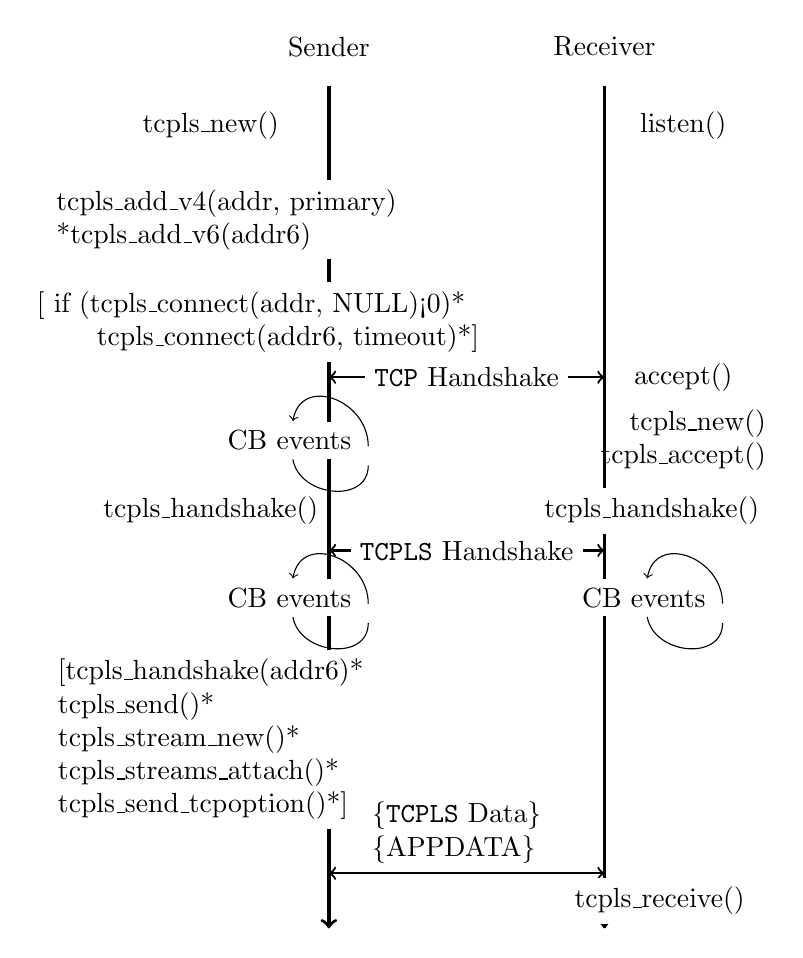
\begin{tikzpicture}
   \colorlet{lightgray}{black!20}
   \tikzstyle{arrow} = [thick,->,>=stealth]
   \tikzset{state/.style={rectangle, dashed, draw, fill=white} }
   \node[black, fill=white] at (0.5,10) {Sender};
   \node[black, fill=white] at (4,10) {Receiver};
   \draw[very thick,->] (0.5,9.5) -- (0.5,-1.2);
   \draw[very thick,->] (4,9.5) -- (4,-1.2);
   \node at (-1,9) {tcpls\_new()};
   \node at (5, 9) {listen()};
   \node[align=left, fill=white] at (-0.8,7.8) {tcpls\_add\_v4(addr,
     primary)\\*tcpls\_add\_v6(addr6)};
   \node[fill=white, align=left] at (-0.4,6.5) {[ if (tcpls\_connect(addr,
     NULL)<0)*\\
     \indent~~tcpls\_connect(addr6, timeout)*]};
   \draw[black, thick, <->] (0.5,5.8) -- (4,5.8) node [midway, fill=white] {\tcp Handshake};
   \node[fill=white] at (0,5) (Callback) {CB events};
   \node at (1,4.8) (here) {};
   \draw [->] (Callback) to[out=-80, in=-90,looseness=1.3] (here)
   to[out=90,in=80,looseness=1.5] (Callback);
   \node at (5, 5.8) {accept()};
   \node[align=right] at (5, 5) {tcpls\_new()\\tcpls\_accept()};
   \node at (-1,4.1) {tcpls\_handshake()};
   \node[fill=white] at (4.6,4.1) {tcpls\_handshake()};
   \draw[black, thick, <->] (0.5,3.6) -- (4,3.6) node [midway, fill=white] {\tcpls Handshake};
   \node[fill=white] at (0,3) (CB2) {CB events};
   \node at (1,2.8) (here2) {};
   \draw [->] (CB2) to[out=-80, in=-90,looseness=1.3] (here2)
   to[out=90,in=80,looseness=1.5] (CB2);
   \node[fill=white] at (4.5,3) (CB3) {CB events};
   \node at (5.5,2.8) (here3) {};
   \draw [->] (CB3) to[out=-80, in=-90,looseness=1.3] (here3)
   to[out=90,in=80,looseness=1.5] (CB3);
   \node[fill=white, align=left] at (-1, 1.2)
   {[tcpls\_handshake(addr6)*\\tcpls\_send()*\\tcpls\_stream\_new()*\\tcpls\_streams\_attach()*\\tcpls\_send\_tcpoption()*]};
   \draw[black, thick, <->] (0.5,-0.5) -- (4,-0.5) node [midway, fill=white,
   above, text width=2.4cm]
   {\{\tcpls Data\} \{APPDATA\}};
   \node[fill=white] at (4.7,-0.85) {tcpls\_receive()};
\end{tikzpicture}
}
\caption{API Workflow example. * means optional call, [ ] means optional call flow, and \{ \} means encrypted.}
  \label{fig:api}
\end{figure}

Fig.~\ref{fig:api} shows an example of our current API workflow. The API can handle explicit multipath techniques such as Happy Eyeball by chaining
\texttt{tcpls\_connect()} with an appropriate timeout of 50ms, as shown in the
Figure. \tcpls lets the application explicitly choose the multipath mesh by calling several times \texttt{tcpls\_connect(src, dest,timeout)};. The application may configure callbacks to connection events that would occur within \tcpls, such as a connection establishment, a stream attachment, a multipath join, the reception of a \tcp option to tune \tcp, and
more. When multiple streams are attached to multiple \tcp connections, the application may configure various \tcpls behaviours. Among them, we support HOL-blocking avoidance, aggregation of bandwidth with multipathing, connection failover, and connection migration. Note that, HOL-blocking avoidance is incompatible with the aggregation of bandwidth with multipathing (the application can do either one but not both at the same time).



%Note, those features are not stable yet, and many bugs remain to be fixed.

\subsection{On \tcp Extensibility}
\label{sec:tcpoptions}

The \tcp specification limits the size of the entire \tcp header (including options) to 64 bytes. Unfortunately, the \tcp designers did not foresee that so many \tcp extensions would be standardized. Today, the size of the \tcp header
becomes a constraint. For example, it severely limits the number of gaps that
can be covered by selective acknowledgments. This gets worse with extensions
such as \mptcp~\cite{rfc6824} that consume more space in the \tcp header.
The IETF has discussed this problem for several years, but the latest attempt
to solve it~\cite{draft-ietf-tcpm-tcp-edo-10} has not yet been implemented by
major \tcp stacks.

\tcpls provides more space for some \tcp options. First, with \tcpls, \tcp
options can be negotiated during the \tls handshake. Since the \tls messages are
included in the \tcp payload, there is more space to carry them. Another
advantage of this approach is that the \tcp options are secured by \tls. This
implies that they cannot be modified by middleboxes. This could be an advantage,
but could also prevent \tcpls from correctly working through some types of
transparent \tcp proxies.

Second, we can also carry \tcp options inside \tls records. For example, we used
this feature to implement the \tcp User Time Out option \cite{rfc5482}. A client
can use this option to set the maximum value of the retransmission
timer on a server. Linux \tcp has a socket option that allows setting
this timer locally, but it does not implement the option. With \tcpls, the client sends the option inside a \tls record, the server extracts it
and performs the required \texttt{setsockopt}.

\subsection{Multipathing}

\subsubsection{Application-level Connection Migration}
\label{sec:connmigr}

Given the availability of multiple IP paths, connection migration might be a
powerful tool to improve the application connection's reliability.  We implement Connection migration and Failover as two distinct measures to handle
two different inquiries: ($i$) The application expects to take advantage of multiple IP paths. ($ii$) The application expects to be resilient to a network outage. In the first case, we implement connection migration and multipathing from a protocol viewpoint, as the same exchange of messages and API calls from \tcpls. It is left for the application to decide and program
through the API calls whether it wants to move all the traffic from one path to
another or split the traffic among the available paths according to any
scheduling policy. The second inquiry focuses on simply configuring \tcpls to automatically move the traffic to another available IP-level path if a network outage is detected.
%The current implementation supports surviving abrupt reset of the connection,
%yet we may also want to
%monitor the connection and switch to another one if the path quality is low.


\subsubsection{Failover}\label{failover}
describing Failover

\subsubsection{Data Aggregation}
Describing orderings and schedulers

\subsection{0-RTT Connections}



\section{\tcpls Evaluation[BUDGET=3p]}
\label{sec:evaluation}
% !TEX root = ./paper.tex

In this section, we evaluate \tcpls using two different types of experiments. First, analyze the raw performance of our \tcpls prototype and the interactions with real middleboxes in a lab with a few servers. We then emulate more complex network scenarios that include failover and multipathing using Mininet~\cite{handigol2012reproducible}. \todo{BD: is it the same ref as the next one (broken)?}


%Our objective is to evaluate whether our design and implementation are indeed
%fast, flexible and does not conflict with several commercial and open-source
%middleboxes. Moreover, we expect to showcase and compare TCPLS's functionalities
%such as the App-level connection migration, the failover mechanism or the
%bandwidth aggregation capability. We discuss them against the state
%of the art designs, such as mvfst~\cite{mvfast}, quicly~\cite{quicly},
%msquic~\cite{msquic}, MPTCP~\ref{mptcp}, pquic~\cite{pquic},
%quic-go~\cite{quic-go} and MPQUIC~\ref{mpquic}.

%TODO do we also evelatuate security? with a simple proof and discussion?

To evaluate \tcpls's functionalities, we rely on reproducible network
experimentations with Mininet~\cite{mininet}. Our objective is to compare the
behaviour of \tcpls with the state of the art, and to make it easily
reproducible for future works, as the quic implementations continue to evolve.

\subsection{Capability Comparison}

Table~\ref{table:tcplsvsquic} compares the features supported by
\tcp, \tls/\tcp, \quic and \tcpls. \quic and \tcpls are very similar in their
capabilities. They mainly differ in their semantic. \tcpls's semantic is to let
the applications make the decision, and we design its API to fulfill this goal.
That is, the meaning of \tcpls is to offer advanced, extensible and secure
transport-layer functionalities on top of \tcp, while exposing a simple but
powerful API to let the application composes the properties its transport should
have.

Note that several of the features suggested by \tcpls are also suggested on \tcp or \quic via research works such as a new socket API for explicit multipath for \tcp\cite{hesmans2016enhanced}, or eBPF plugins in
\quic~\cite{de2019pluginizing}.

\begin{table}
  \small
  \begin{tabular}{lcccc}
    \toprule
    & \tcp & \tls/\tcp & \quic & \tcpls \\
    \midrule
    Transport reliability & \checkmark & \checkmark &
    \checkmark & \checkmark \\
    Message conf. and auth.&  \xmark & \checkmark & \checkmark & \checkmark \\
    Connection reliability (failover) &  \xmark & \xmark & (\checkmark) & \checkmark \\
    0-RTT & \checkmark & (\xmark) & \checkmark  & \checkmark \\
    Session Resumption & \xmark & \checkmark & \checkmark & \checkmark \\
    Connection Migration & \xmark & \xmark & \checkmark & \checkmark \\
    \multicolumn{5}{l}{Application-exposed features} \\
    \hspace{2em} Streams & \xmark & \xmark & \checkmark & \checkmark \\
    \hspace{2em} Happy eyeballs & \xmark & \xmark & \xmark & \checkmark \\
    \hspace{2em} Explicit Multipath & \xmark & \xmark & \xmark & \checkmark \\
    \hspace{2em} App-level Con. migration & \xmark & \xmark & \xmark & \checkmark \\
    \hspace{2em} Pluginization & \xmark & \xmark & \xmark & (\checkmark) \\
    Resilience to HOL blocking & \xmark & \xmark & \checkmark  & \checkmark \\
    Secure Connection Closing & \xmark &  \xmark & \checkmark & \checkmark \\
    \bottomrule
  \end{tabular}
  \caption{Protocol features comparison. (\xmark) means that the feature is
    available, but not straightforward to use. (\checkmark) means that the
  feature is partially available and under development.}
  \label{table:tcplsvsquic}
\end{table}

\subsection{Raw Performance}
\label{sec:perf}

To evaluate the raw performance (Sec.~\ref{sec:perf}) and middlebox traversal
(Sec.~\ref{sec:middlebox}) of our \tcpls prototype, we use the testbed shown in Fig.~\ref{fig:perf_testbed}. It contains three servers equipped with Intel Xeon CPU E5-2630 2.40GHz, 16 Threads, at least 16GB RAM, running Debian with Linux 5.9 and 5.7 kernels. Two of these machines are used as Client and Server,
while the third one is used as a router or a middlebox. Each machine is equipped with an Intel XL710 2x40GB NIC. With Jumbo frames, a single \tcp connection can saturate the 40 Gbps path. With a 1500 bytes MTU, a single connection reaches 22 Gbps.

\begin{figure}[!t]
  \begin{center}
    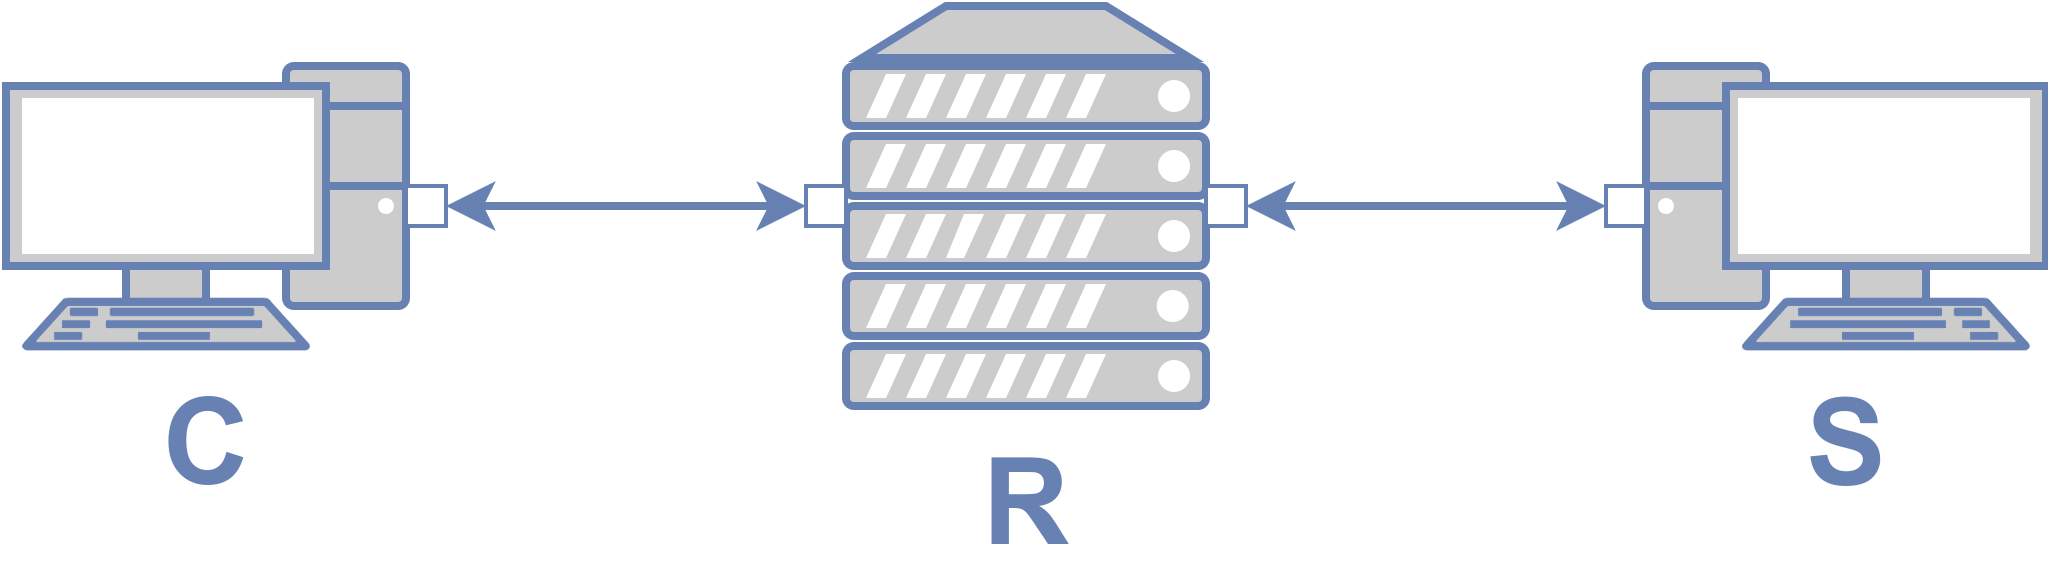
\includegraphics[width=6cm]{figures/testbed.png}
  \end{center}
  \vspace{-0.5cm}
  \caption{
    Performance Measurements Setups. C = Client. S = Server. R = Router/Middlebox.}
  \label{fig:perf_testbed}
    \vspace{-0.5cm}
\end{figure}


The first question that we want to answer is whether \tcpls can compete with the traditionnal \tls over \tcp stack. We then compare our \tcpls prototype with different \quic implementations.


\paragraph*{\tcpls}
For all the \tcpls measurements, we used a custom application that performs large memory-to-memory transfers over a \tcpls session using a single stream. \tcpls was configured to use the \todo{AES-...} encryption scheme.
Fig.~\ref{fig:perf} provides the goodput measured in our testbed. We report both the bandwidth in megabits per second and packets per second.  Each bar in this figure is the average over \todo{x} runs. The bottom bar is the highest goodput that we measured with \tcpls: \todo{12 Gbps}. This result was obtained with jumbo frames (i.e. 9000 bytes MTU) and using TCP Segmentation Offload (TSO) on the NICs. TSO is a standard feature that is enabled by all high-speed NICS. The next bar shows that with TSO and a standard frame size (1500 bytes MTU), the goodput is still \todo{11 Gbps}. These results should be compared with the 22~Gbps that TCP reaches in the same environment using \texttt{iperf} but without any encryption. We measured that \todo{AES-...} peaks at \todo{xx} Gbps when doing in-memory encrytion/decryption on our testbed's servers.

%the
%shows several interesting results. First, while
%offering similar (and more) capabilities than what QUIC is providing today,
%\tcpls is also more than twice faster than the strongest evaluated QUIC
%implementation (quicly) over CPU limited experimentations. We evaluate \tcpls

We then evaluated the impact of adding the \tcpls-level acknowledgements
described in Sec.~\ref{failover} to support failover.
% Thanks to these acknowledgements, \tcpls can support failover.
From a performance viewpoint, they increase the number of control records and the number of system calls. Our prototype currently sends a \tcpls-ack for every 16 received records, or after having received 15 times the maximum \tls payload \todo{OB ne voit pas la différence}, or upon the expiration of \todo{xx msec} timer. Our measurements indicate that with this functionnality, \tcpls reaches \todo{9.5 Gbps}.


\begin{figure}[!t]
  \begin{center}
    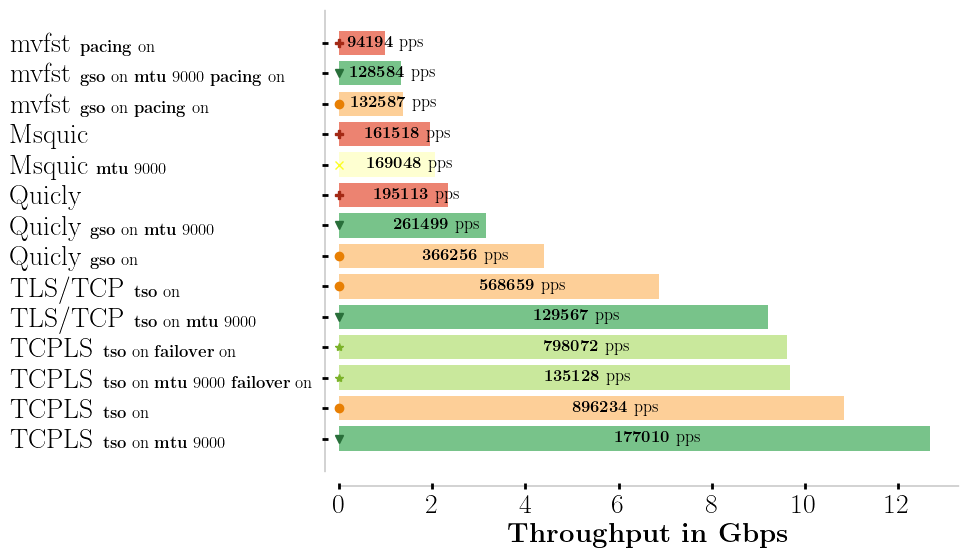
\includegraphics[width=\columnwidth]{figures/perf_analysis.png}
  \end{center}
  \caption{The \tcpls prototype is faster than \tls over \tcp and different \quic implementations.}
  \label{fig:perf}
\end{figure}


%in four different settings: with a path mtu of 1500 or 9000, and with failover
%enabled or not. The failover functionality is an internal stack feature that
%provides session reliability, which increases the number of syscalls that TCPLS
%makes by exchanging TCPLS-level record acknowledgments. We currently send an ac%k
%for
%throughput at the price of a slower recovery in case of network failure.

\paragraph*{\tcpls vs. \tls/\tcp}
We now compare the performance of \tcpls with the traditional \tls over \tcp stack. To have a fair comparison, we use \texttt{picotls}'s client/server
implementation with the same commit as our initial fork for \tcpls.
\todo{test client pour TLS/TCP}
Fig.~\ref{fig:perf} shows that \tls/\tcp provides a lower performance than
\tcpls with regular and jumbo frames. This can be explained by the receiving
buffer size provided to \texttt{read()}, which is hardcoded to 16,384 bytes
\todo{in \texttt{picotls}}. This implementation results in fragmentation on the
receiver and prevents it from using the zero-copy code path provided by the
library. \tcpls uses a larger read buffer and benefits from zero-copy. At first, one may consider this as an unfair comparison, however the devil is in the details. In \tcpls implementation, the application developers cannot touch \texttt{read()}'s interface. This implies that an application developer cannot missuse the relationship between \tls and \tcp by creating fragmented records and doing unecessary copies to handle those fragments. \tcpls's design and implementation try to prevent fragmentation by first, having a sufficiently large read buffer size. Second, \tcpls only starts deciphering a record it has received the entire record. \tls/\tcp record fragmentation is provided by TLS libraries as a usability feature that spares the application developers from taking into account all \tls details, at the cost of lower performance.
With \tcpls application developers can ignore \tls details without missusing the interface, which is the reason why this comparison is interesting.\tcpls constrains the application developer to use the buffer type provided
by the API, but offers zero-copy deciphered records in return.

%\todo{OB: pas sur que la suite est nécessaire} Moreover, but this has not
%yet been implemented, it could be interesting to match the TLS record size to
%the congestion window to deliver faster the data to the application when the
%network is congested.

\paragraph{\tcpls vs. \quic}
Although \quic~\cite{draft-ietf-quic-transport} is a young protocol, there are
already more than a dozen implementations~\cite{marx2020same,quicimplem,yang2020making} under active development. We compiled and installed three representative \quic implementations in our testbed: Facebook's mvfst~\cite{} from Facebook, Microsoft's msquic~\cite{} Fastly's quicly~\cite{}. They are all developed by
large companies that (plan to) use them in production and include their own
benchmarking application to perform throughput measurements. Furhtermore,
mvfast and quicly support Generic Segmentation Offload (GSO), which should improve performance by offloading \udp segmentation and checksum computation available on our NICs. We use the implementation's bechmarking application
as is, exploiting the optional arguments provided by their interface to increase the throughput but drawing the line there. That is, we do not modify the QUIC implementations.

The results shown in Fig.~\ref{fig:perf} show that \tcpls compares favorably
with the tested \quic implementations. The fastest \quic implementation is quicly. Thanks to GSO, it reaches \todo{4 Gbps} in our testbed with a 1500 bytes MTU. This result is directly comparable to \tcpls with TSO enabled,
which still performs more than twice faster at 100\% CPU peak with similar configurations for the transport parameters. Suprisingly, quicly's performance decreases with jumbo frames but is still faster than when GSO is disabled. In our testbed, msquic could only reach \todo{2 Gbps} and mvfst was slower.


%QUIC is young protocol, and all implementations are in active development, with
%different states for their available features and optimizations. For example,
%none of the implementations were able to take advantage of a path mtu larger
%than 1500, and it even degraded the performance in the case of quicly. Two of them
%(quicly and mvfst) have implemented the support for \texttt{gso} leading in the
%case of quicly to more than 4 gb/s of throughput with a udp payload length
%configured to match TCP (1460).


%We perform a throughput evaluation of \tcpls and compare it to several major
%QUIC implementations: mvfst~\cite{} from Facebook, msquic~\cite{} from Microsoft
%and quicly~\cite{} from Fastly. Our choice of QUIC implementations was mainly
%influenced by the availability of a client/server perf tool specifically
%engineered for a throughput evaluation. A second criterion was the advancement
%of the implementation and the quality of the code. We hope to avoid most of the
%bugs negatively impacting their results by selecting the QUIC implementation
%that show advanced features and testings. A third criterion was the development
%language used. \tcpls is written in C, and we prefer to compare it against QUIC
%implementation written in a language compiled by clang or gcc. Mvfst, msquic
%and quicly meet these criteria.



\subsection{Middlebox Interferences}

When deploying a novel protocol, different middlebox interferences may arise
depending on the changes introduced in the packets wire image. In this
regard, \tcpls comes with two novel \tls extensions: \tcpls and \join.
We discuss the potential issues and countermeasures below.

If a clients attempts to open a \tcpls to in the presence of a \tls termination
proxy or bridging proxy, it sends a \textsc{ClientHello} that includes
the \tcpls extension.
If the proxy does not support \tcpls, it replies with a \textsc{ServerHello}
message that does not include the \tcpls extension. From this point, the client
implicitely fallback to \tls, and continues with the handshake.

Certain legacy \tls server implementations are known not to implement the \tls
specification properly and might abort connections when receiving unknown \tls
extensions. Analogous behavior has been observed in overly restrictive stateful
firewalls.  To ensure connectivity in the presence of such policies, \tcpls
implements an explicit fallback mechanism. If a device sends a \tcp \rst in
response to the \tcpls-setup \textsc{ClientHello}, or silently discards it,
the client attempts at negotiating a second non-\tcpls \tls connection, either
immediately or after a timeout. Similarly, a \tcpls \join extension might be
blocked on the path. In this case, the subflow attachment is canceled, and
the application is directly notified to be able to react appropriatly (e.g.,
to cancel a migration attempt).

We tested \tcpls against opensource and commercial stateful firewalls and proxy
implementations and (i.e., pfSense, IPFire, Cisco ASAv, mitmproxy) and found no
interferences. Still, certain middlebox security appliances that implement
pervasive monitoring allows for configurable TLS extensions blocking
\cite{rfc7258}. This is handled properly by \tcpls fallback mechanism.


\subsection{Bandwidth Aggregation}

\begin{figure}[!t]
  \begin{center}
    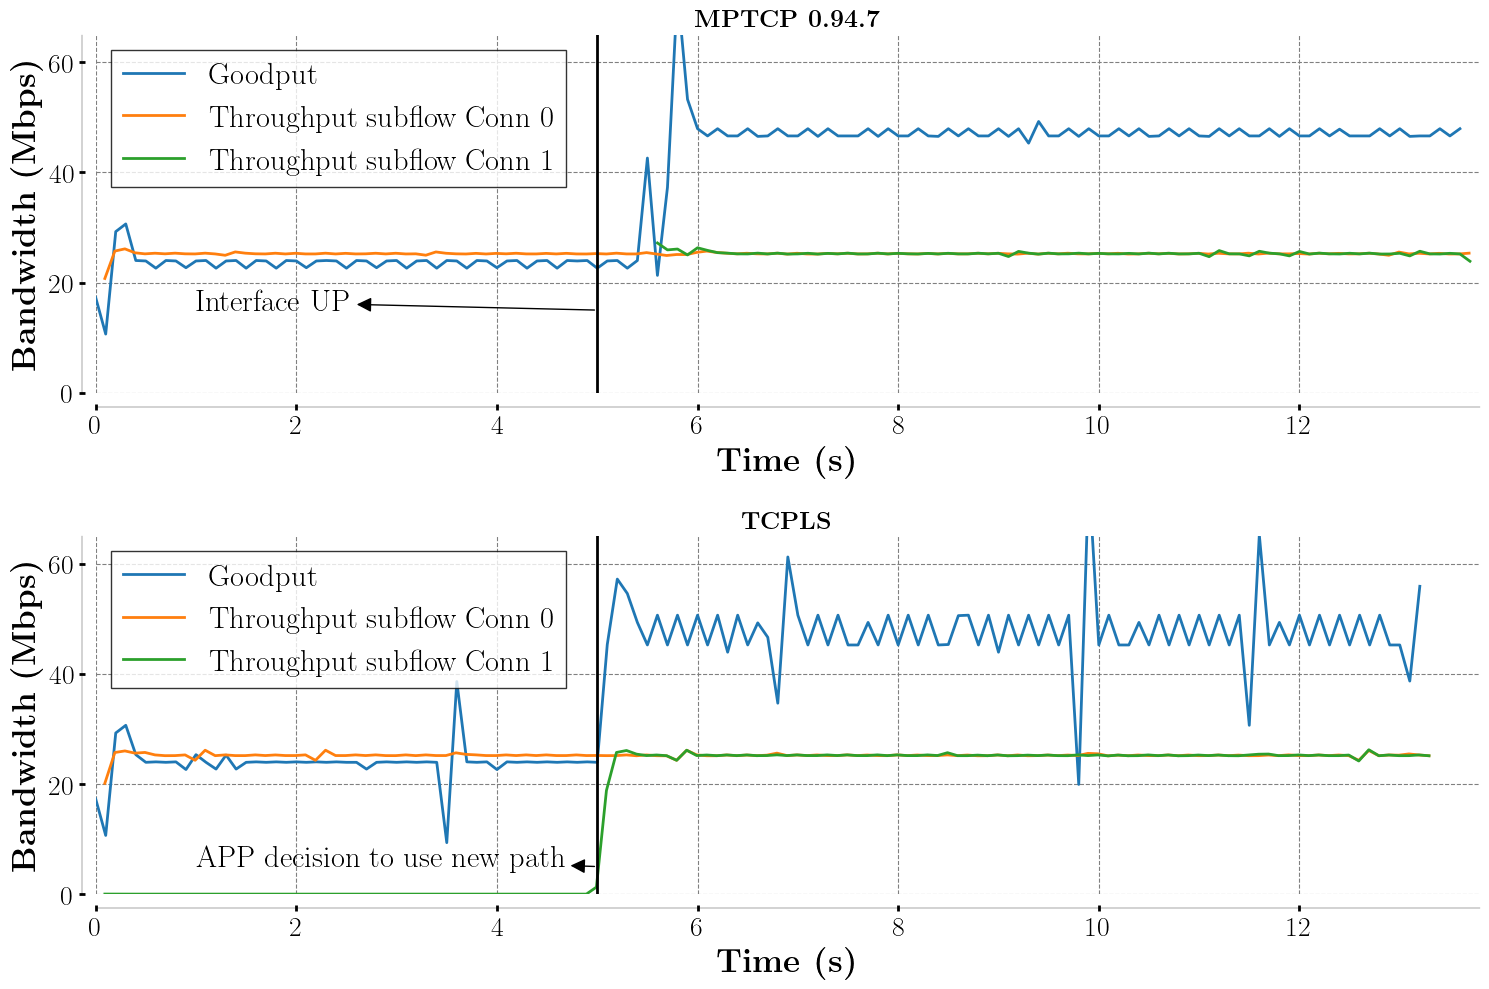
\includegraphics[width=\columnwidth]{figures/aggregate_dual.png}
  \end{center} \
  caption{Bandwidth aggregation comparison between \mptcp and
    \tcpls.}
\end{figure}

\subsection{Application-Level Migration}


Detailler pourquoi on a besoin du controle applicatif pour la migration, et à
quels cas du monde réels ils s'appliquent


Fig.~\ref{fig:conn_migration} shows the result of an Application-level
connection migration demo using the API (i.e., it is left to the
application to decide when to migrate, and we expose a simplistic code flow to
perform it). In this experiment, we use an IPMininet network~\cite{ipmininet, jadin2020educational} \todo{BD: Mininet above, IPMininet here with different refs.  Make sure to be consistent}
composed of a client and a server, both dual-stacks. One path within the
network is composed of OSPF routers with IPv4 only, and one path is composed of
OSPF6 routers IPv6 only. We configure the bandwidth to 30Mbps, the lowest delay
to the v4 link. Our application downloads a 60 MB file from a server and migrates to the v6 connection in the middle of the download.

Triggering the connection migration involves chaining 5 API calls:
first, \texttt{tcpls\_handshake()} configured with handshake properties announcing a \join over the v6 connection id. Then, the creation of a new stream
\texttt{tcpls\_stream\_new()} for the v6 connection id, finally followed by the attachment of this new stream \texttt{tcpls\_streams\_attach()} and the secure closing of the v4 \tcp connection using \texttt{tcpls\_stream\_close()}. Following these events, the server seamlessly switches the path while looping over \texttt{tcpls\_send} to send the file content. Note that all the events trigger callbacks on the server side, to let the server react appropriately if other requirements need to be fulfilled.

\tcpls's application connection migration takes advantage of multipath to offer
a smooth handover to applications, which \tcpls cannot do at the moment.

\begin{figure}[!t]
  \centering
  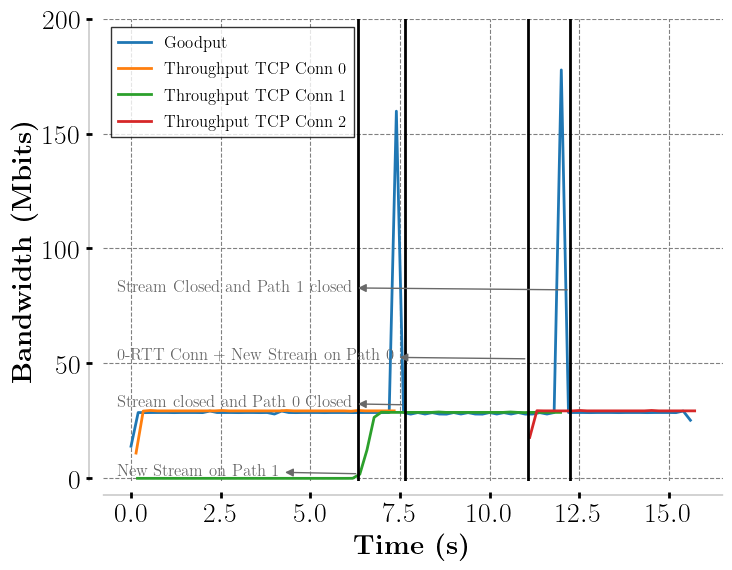
\includegraphics[width=6cm]{figures/migration.png}
  \caption{Application-level connection migration during a 60MB file download.}
  \label{fig:conn_migration}
\end{figure}

\subsection{Failover}

1) analyse du temps de recovery pour different type de cassure, et comparaison avec mptcp
2) discuter une propriété de "connection reliability" => ca casse, on restabilise le plus vite possible
3) montrer que le path manager est important pour cette propriété, et que ce n'est pas encore au point pour mptcp, mpquic, etc

Mptcp overhead: 1.0744997978210449
TCPLS overhead: 1.0994282363439873
MPTCP overhead/TCPLS overhead:              0.9773259975513828


\begin{figure}[!t]
  \begin{center}
    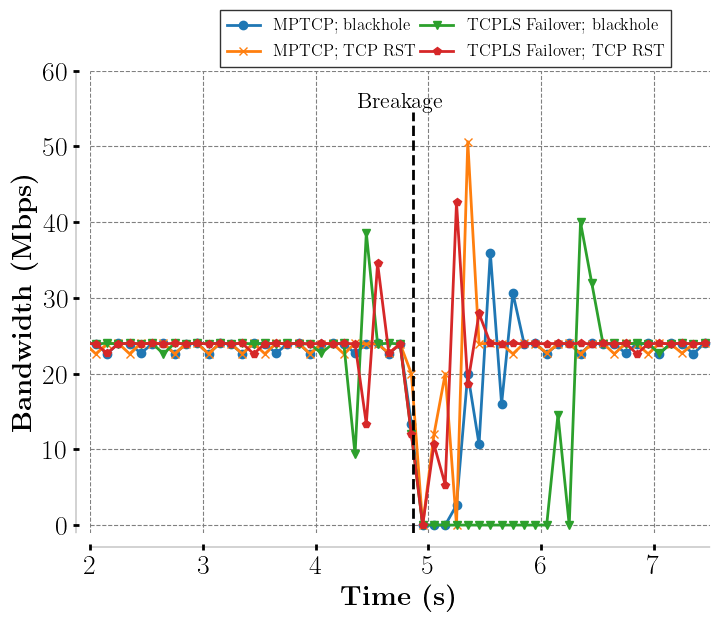
\includegraphics[width=6cm]{figures/breakage_analysis.png}
  \end{center}
  \caption{Recovery speed analysis.}
\end{figure}


\begin{figure}[!t]
  \begin{center}
    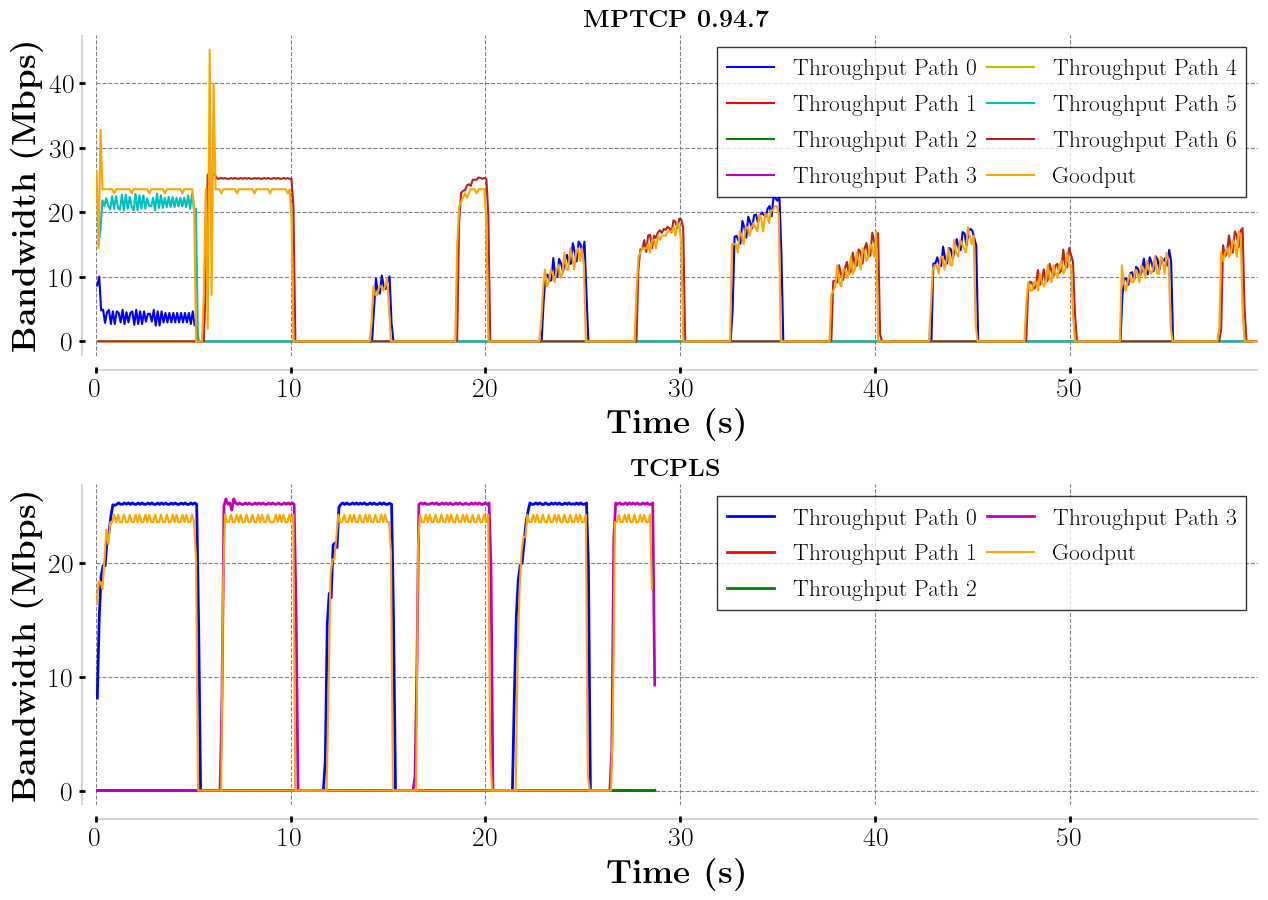
\includegraphics[width=6cm]{figures/tcpls_mptcp.png}
  \end{center}
  \caption{Connection reliability: influence of the path manager and congestion
  control.}
\end{figure}



\subsection{Dynamically Extending \tcpls}

The \tcpls streams enable new use case. Obviously, a \tcpls application can
create and use different streams to carry data. However, since these streams
are generic, they can also be used by the \tcpls implementation itself to
exchange control information. To demonstrate the versatily of these control
streams, we extended \tcpls to enable a server to push a different congestion
control scheme to a specific client over an existing \tcpls session. Recent
work on restructuring congestion control has proposed a generic architecture
for congestion controllers \cite{narayan2018restructuring}.
During the last years, the Linux kernel developpers have relied on eBPF
to make the Linux TCP/IP stack \cite{brakmo2017tcp,tran2020beyond} easier
to extend. Since Linux kernel version 5.6, an application can inject
a different congestion control scheme entirely implemented using eBPF. A similar approach was proposed in Pluginizing \quic~\cite{de2019pluginizing}.
We leverage these new eBPF capabilities to demonstrate the feasibility of injecting and updating a congestion control scheme during a \tcpls session.

We perform our experiment using Mininet \todo{BD: same remark as above.  Mininet or IPMininet} over a 100 Mbps emulated link that has a 60 msec delay. Fig.~\ref{fig:vegasCubic} shows a client that uses the TCP Vegas~\cite{10.1145/190314.190317} congestion control scheme to upload a file. This \tcpls session fully uses the bottleneck link. After some time, another client starts an upload, but using the CUBIC congestion controller~\cite{rfc8312}. This results in an unfair distribution of the bandwidth. The server then sends the eBPF bytecode of the CUBIC congestion control scheme to the TCP Vegas client that injects it in its kernel and the unfairness disappears.  We performed the same experiment for different delay, varying from 10ms to 100ms.

\begin{figure}[!t]
  \begin{center}
    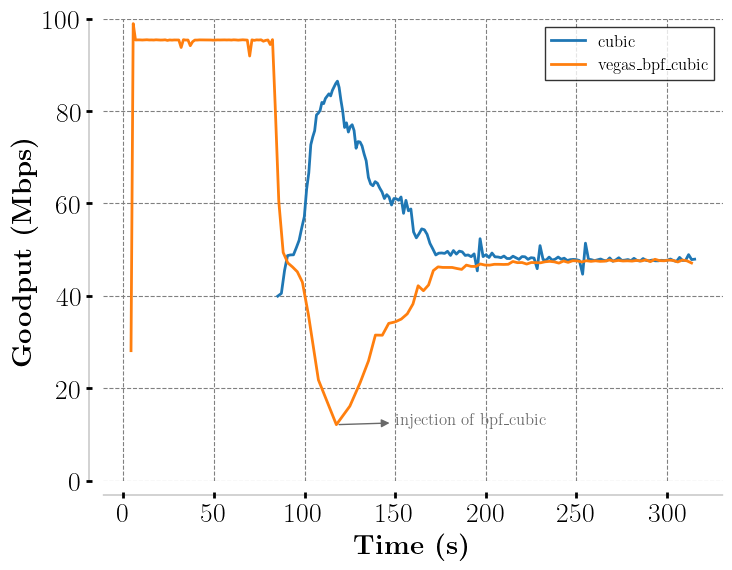
\includegraphics[width=6cm]{pretty_plotify/plots/vegas_cubic.png}
  \end{center}
  \caption{\tcpls hosts can exchange congestion control schemes and activate them during a \tcpls session.}
  \label{fig:vegasCubic}
\end{figure}


\section{Conclusion[BUDGET=0.5]}
\label{sec:conclusion}
% !TEX root = ./paper.tex
\tcp and \tls were designed as independent protocols, but they are very often
used together. In this paper, we have shown that this is possible to design and
implement the \tcpls protocol that is fast, flexible, and secure by closely
coupling \tcp and \tls.

\tcpls inherits the security features of \tls 1.3 and all the reliability and
congestion control techniques that have been added to \tcp during the last
decades. More specifically, \tcpls extends the \tls 1.3 handshake and the record
layer to create a secure control channel between the two communicating hosts.
The messages exchanged over this channel are placed inside \tls records that are
encrypted and authenticated and also hidden from middleboxes. \tcpls leverages
these control messages to support fast failovers, smooth
migration of the \tcpls session from one path to another and to provide
bandwidth aggregation under full control of the application through an API. 
\tcpls can also use the secure channel to extend \tcp with new options and even
use the \tcpls session to exchange a different congestion control scheme that
is then used for this session.

Thanks to \tcpls's design, our \tcpls implementation provides a
flexible API that allows the applications to perform zero-copy data transfers,
and easily manipulate the different features presented in this research work.
The performance evaluation shows that our prototype is more than twice as fast
as currently available \quic implementations while supporting additional
features such as bandwidth aggregation and stream steering.

\tcpls is both simple and powerful. Simple because it can be implemented inside
existing \tls libraries without any kernel change in contrast to \mptcp. \tcpls 
is
wire-compatible with the existing \tcp middleboxes and can thus be used in all
environments where \tls 1.3 is used over \tcp. Given the performance benefits of
\tcpls, the flexibility it offers and the features that it already provides, we
believe that it can be a powerful contender to \quic for modern services, 
including HTTP.



%\section{Implementation, Deployment \& Research Questions}

%% !TEX root = ./paper.tex

A \texttt{TCPLS} reference implementation is under active development. The
current implementation is forked from a fast and full
TLS 1.3 implementation written in \texttt{C}. It currently adds about 5k lines
of code (including unit tests and inline code comments) compared to the upstream branch.

The current implementation offers:
\begin{inparaenum}
  \item An experimental API that wraps TLS and TCP
  \item Our design of TCP's extensibility mechanism throught TCP option sent
within TLS records and processed by TCPLS. We currently support TCP User
Timeout and the injection of eBPF bytecode for TCP's congestion control
algorithm. Supporting another TCP option is only a matter of extending the sender's
API and processing the option
on the receiver side. TCPLS's internal machinery is already implemented for any
type of TCP option to send during the handshake or when the handshake completed.
  \item The support of parallel streams and multiplexing over TCP connections.
    Each stream has its own cryptographic context.
  \item Connection migration and multipathing.
\end{inparaenum}

We expect to investigate several research questions with TCPLS. First, we are
interested in analyzing how far we can go into supporting TCP's extensibility
through our mechanism. Several of new TCP features may require to inject eBPF
bytecode to the kernel. It is still unclear how much of TCP could be extended,
and if \texttt{TCPLS} may play a role in incentivizing the linux kernel's maintainer
to support more eBPF in TCP's implementation, since we now offer a technique to
propagate eBPF bytecode within authenticated and confidential session with a
trusted server.

Second, we expect to analyze several features of TCPLS, such as our
connection migration, our multipath implementation and our failover mechanism.
Answering the question about how much TCPLS can or and how fast it performs in
case of a migration or a network outage.

Finally, we would expect to critisize QUIC in light of our \texttt{TCPLS}
design. We will compare both QUIC and TCPLS, discuss the differences, and analyze
and answer questions regarding the requirements in transport protocol for today's
Internet applications.


%\section{Related Work}

%% !TEX root = ./paper.tex

By combining \tcp and \tls, \tcpls builds upon two of the most important
Internet protocols. Given their importance within  the research community and the IETF, we restrict our discussion to close related works. Readers may refer to survey papers for additional  context
information~\cite{polese2019survey,li2016multipath,papastergiou2016ossifying}.

Regarding its transport features, \tcpls' stream abstraction has similarities to
the Structured Streams Abstraction~\cite{ford2007structured}, in which each
stream does not need 3-way handshaking, is independent if attached to a
different \tcp connection and can proceed in parallel without head-of-line
blocking if the streams are not coupled. However, \tcpls pushes further the
abstraction, involving benefits leveraged from multiple connections.

\tcpls uses \tls records to encode data and control information. Researchers
have also explored the idea of encoding control information in the \tcp
bytestream in different protocols. During the initial discussions for Multipath \tcp, Multi-Connection \tcp (\texttt{MCTCP})~\cite{draft-scharf-mptcp-mctcp-01}
was proposed as an alternative that encodes control information in the bytestream. The \mptcp Working Group did not adopt this solution because it notably feared of possible problems with middleboxes. Multipath \tcp~\cite{raiciu2012hard,rfc8684} uses \tcp Options to encode control information and use different paths. \tcpls uses \tls records for this purpose and prevents middlebox tampering. Since \tls records are encrypted, their integrity protected, and protocol-level indistinguishable, middleboxes cannot interfere with the control information that \tcpls exchanges. In contrast, with \mptcp, a middlebox that modifies the payload, such as a transparent \tcp proxy or an application level gateway running on a NAT~\cite{rfc3027}, can disrupt the
protocol. Minion~\cite{nowlan2012fitting} also encodes control information in
the \tcp payload but to support unreliable data.

Given its security features, \tcpls must be compared with
\tcpcrypt~\cite{bittau2010case,rfc8548} which predates \tls 1.3. It uses \tcp
options to support opportunistic encryption but is not secure against an active
network attacker. \tcpls extends \tls while retaining its security  properties, 
and supporting new features. It is also compatible with middleboxes, as it 
leaves the \tcp wire format untouched.

%\tcpls also needs to be compared with
%\mptcp \cite{raiciu2012hard,rfc6824}.
\mptcp \cite{raiciu2012hard,rfc6824} supports several coupled congestion
control schemes \cite{peng2014multipath,wischik2011design,khalili2013mptcp}
that preserve fairness when different paths share the same bottleneck. A
similar solution  could be applied to \tcpls by leveraging eBPF to access and
modify the  congestion controller state. We leave this engineering effort as
future work. The initial idea of coupling \mptcp and \tls was proposed in an
Internet draft~\cite{draft-paasch-mptcp-ssl-00} that was not adopted by the
IETF. MPTCPSec~\cite{jadin2017securing} adds security capabilities to \mptcp but
comes with a large performance penalty.

Another important related work is \quic. %Its design has
%evolved over the years, and several companies adopted
%it~\cite{langley2017quic,Joras_mvfst,marx2020same}.
\quic version 1~\cite{rfc9000} also supports connection migration, but to our 
knowledge current implementations do not allow applications to trigger  it. 
%outside 
%from limited interoperability scripts.
%we could not test it in our lab since none of
%the available open-source implementations have implemented it yet.
Multipath extensions
\cite{viernickel2018multipath,de2017multipath,draft-liu-multipath-quic-02,I-D.lmbdhk-quic-multipath}
to \quic have been discussed but not yet adopted within the IETF. Finally,
\texttt{PQUIC}~\cite{de2019pluginizing} proposed to convey eBPF code over \quic
connections to deploy new protocol features. The same benefits are also being
considered for other distributed systems, such as BGP~\cite{xBGP} and
anonymous overlay networks~\cite{fan-hotpets}. This goes beyond the exchange of 
a congestion controller in \tcpls.

Finally, several solutions have been proposed to provide multipath capabilities
in the application layer. Examples include MP-H2~\cite{nikravesh2019mp} that
extends HTTP/2, MP-DASH~\cite{han2016mp} for video streaming or mHTTP~\cite{kim2014multi} that extends HTTP.

\tcpls also share similarities with \tls FOP~\cite{sy2020enhanced}, which
solves the privacy issue with TFO by using \tls. However, \tcpls is more 
generic, and its extensibility enables more advanced concerns and transport 
services.

%% Several researchers have proposed techniques to extend various transport
%% protocols. The IETF provides generic guidelines on the design of
%% protocol extensions \cite{rfc6709}. Several researchers have proposed
%% solutions to simplify the implementation of extensions to transport
%% protocols. The closest example include STP \cite{patel2003upgrading}, CTP
%% \cite{bridges2007configurable} and

%% Patel et al. \cite{patel2003upgrading} propose to use a type-safe version of C to extend a TCP
%% implementation by using bytecode. The implementation of TCPLS completely differs since it uses C to generate eBPF code. Furthemore, by leveraging the
%% flexibility of TLS, TCPLS can securrely exchange various options over a
%% connection. Bridges et al.
%% In CTP, Bridges et al. propose a new protocol that is composed of different microprotocols which can be combined together. In PQUIC, De Coninck et al. \cite{de2019pluginizing} include an eBPF virtual machine inside a QUIC implementation to extend it by using protocol plugins. Our approach is similar from an implementation viewpoint. By combining the TLS and TCP layers, we bring more extensibility to TCP.

%% %maybe
%% % ictcp \cite{wong2001configurable}

%% %configurable and extensible transport \cite{wong2001configurable}

%% % other protocols maybe

%% The IETF has developed various transport protocols, including
%% DCCP \cite{kohler2006designing}, SCTP \cite{rfc4960} and QUIC \cite{draft-ietf-quic-transport}. DCCP brings more flexible congestion control schemes

%% , lots of research but nothing related \cite{nowlan2012fitting}




%% % maybe
%% % Structured streams \cite{ford2007structured}


%% %TCP papers
%% %generic on extensibility

%% %tcp unreliable

%% A wide range of TCP extensions have been proposed \cite{rfc7414}. Some tune
%% protocol implementations with new strategies to retransmit lost data,
%% compute retransmission timers or manage congestion. These do not require
%% the definition of new TCP options that are negotiated during the handshake.
%% Some TCP extensions require the definition of new TCP options. These
%% include the timestamp and large windows extension \cite{rfc7313},
%% the support for selective acknowledgements \cite{rfc2018}, TCP Fast Open
%% \cite{rfc7413} or Multipath TCP \cite{rfc6824}. These extensions are negotiated
%% by exchanging TCP options during the connection handshake. These TCP options
%% allow to extend TCP, but they suffer from several limitations. First,
%% there is limited space in the TCP header to carry them. This limits the
%% number of extensions that can be used for a given TCP connection. The IETF
%% discusses solutions to extend the TCP header space, but the solution is neither
%% finalized nor implemented \cite{draft-ietf-tcpm-tcp-edo-10}. Second, middleboxes
%% interfere with the utilization of new options \cite{honda2011still}. This
%% interference severely limits the extensibility of TCP. TCPLS does not suffer
%% from these problems since the options that it carries are encrypted and can
%% span an entire TLS record (16KBytes).


%% % \cite{nowlan2012fitting}
%% %TODO
%% % idée de combiner des infos de TLS dans MPTCP
%% %\cite{draft-paasch-mptcp-ssl-00}
%% %\cite{jadin2017securing} % secure mptcp


%\section{Discussion}

%\input{discussion}


\newpage

\section*{Software Artefacts}
%\todo{BD: this section breaks the submission anonymity.  I would, at this step, only considered what I have written in the intro.}

We will release a detailed description of \tcpls and a reference implementation
together with the camera-ready version of the paper. To preserve anonimity,
we cannot provide additional details here. 

%is under active development. The
%current specifications and code are available on
%\url{https://pluginized-protocols.org/tcpls}, forked from a fast and
%full TLS 1.3 implementation written in \texttt{C}. Our \tcpls prototype adds
%about 5k lines of C code to \texttt{picotls} latest version based on the latest
%specification of TLS 1.3.

%\section*{Acknowledgments}
%We thanks the anonymous reviewers for their helpful feedback, and Mathieu Jadin
%for its helpful guidance with IPMininet. This research is supported by the Walloon
%Region through the ``Programme de recherche d'interet general
 %WALINNOV" - MQUIC project (convention number 1810018).


\bibliographystyle{ACM-Reference-Format}
\bibliography{reference}

\appendix
\label{sec:appendices}

% !TEX root = ./paper.tex


%% \section{Sample \tcpls sessions}

%% \tcpls defines several messages that \tcpls hosts can exchange during a \tcpls session. Each of these messages is placed inside an encrypted and authenticated \tls record with a dedicated True Type. The following \tcpls messages are defined in our prototype:

%% \begin{itemize}

%% \item BPF: this \tcpls message contains eBPF bytecode which can be injected in the TCP stack of the receiving host
%% \item MULTIHOMING\_v6: this \tcpls message contains an IPv6 address
%% \item MULTIHOMING\_v4: this \tcpls message contains an IPv4 address
%% \item SESSID: this message contains a variable length identifier for the current \tcpls session
%% \item COOKIE: this \tcpls message contains a cookie
%% \item MPJOIN: this \tcpls message contains \tcpls session identifier and a cookir
%% \item DATA\_ACK: this \tcpls message contains the sequence number of the last record  received over the session
%% \item FAILOVER: \todo{explain}
%% \item FAILOVER\_END: \todo{explain}
%% \item STREAM\_ATTACH: this \tcpls message attaches the stream identifier provided as parameter to the \tcpls session
%% \item STREAM\_CLOSE: this \tcpls message detaches the stream identifier provided as parameter from the \tcpls session
%% \item STREAM\_CLOSE\_ACK: this \tcpls message confirms that the stream identifier provided as parameter has been detached from the \tcpls session
%% \item USER\_TIMEOUT: this \tcpls message encodes the TCP User Timeout option defined \cite{rfc5482}
%% \item TRANSPORT\_NEW: \todo{explain}
%% \item TRANSPORT\_UPDATE: \todo{explain}

%% \end{itemize}

%% We now provide some sample \tcpls sessions to illustrate the operation of the protocol.


%\section{Capability Comparison}


%Table~\ref{table:tcplsvsquic} compares the features supported by \tcp, \mptcp, \tls/\tcp, \quic and \tcpls. \quic and \tcpls are very similar in their capabilities. They mainly differ in their semantic. \tcpls's semantic is to let the applications make the decision, and we design its API to fulfill this goal. That is, the meaning of \tcpls is to offer advanced, extensible and secure transport-layer functionalities on top of \tcp, while exposing a simple but powerful API to let the application decide the properties its transport should have.

%Note that several of the features included in \tcpls are also suggested by researchers for \tcp or \quic such as a new socket API for explicit \mptcp \cite{hesmans2016enhanced}, eBPF plugins in \quic~\cite{de2019pluginizing} or multipath extensions to \quic~\cite{viernickel2018multipath,de2017multipath,draft-liu-multipath-quic-02}.

%\begin{table*}[!t]
%  \small
%  \begin{tabular}{lccccc}
%    \toprule
%    & \tcp & \mptcp & \tls/\tcp & \quic & \tcpls \\
%    \midrule
%    Transport reliability & \checkmark & \checkmark & \checkmark & \checkmark & \checkmark \\
%    Message conf. and auth.&  \xmark & \xmark & \checkmark & \checkmark & \checkmark \\
%    Connection reliability (failover) &  \xmark & \checkmark &\xmark & (\checkmark) & \checkmark \\
%    0-RTT & \checkmark & (\checkmark) & (\xmark) & \checkmark  & \checkmark \\
%    Session Resumption & \xmark & \xmark & \checkmark & \checkmark & \checkmark \\
%    Connection Migration & \xmark & \xmark &\xmark & \checkmark & \checkmark \\
%    \multicolumn{5}{l}{Application-exposed features} \\
%    \hspace{2em} Streams & \xmark &  \xmark & \xmark & \checkmark & \checkmark \\
%    \hspace{2em} Explicit Multipath & \xmark & \xmark & \xmark & \xmark & \checkmark \\
%    \hspace{2em} App-level Con. migration & \xmark & \xmark & \xmark & (\checkmark) & \checkmark \\
%    Resilience to HOL blocking & \xmark & \xmark & \xmark & \checkmark & \checkmark \\
%    Secure Connection Closing & \xmark &  \xmark & \xmark & \checkmark & \checkmark \\
%    \bottomrule
%  \end{tabular}
%  \caption{Protocol features comparison. (\xmark) means that the feature is available, but not straightforward to use. (\checkmark) means that the feature is partially available and under development. \checkmark means that the feature is available, and \xmark means that it is not.}
%  \label{table:tcplsvsquic}
%\end{table*}

%\section{Failover Protocol}
%\label{app:failover}
%Fig.~\ref{fig:protocol_example} provides a closer look at the operation of 
%\tcpls. It
%shows the key \tcpls messages that are exchanged during a \tcpls session using 
%failover
%that transfers a file but suffers from a failure. First, during the \tcpls
%handshake, we observe the \tls encrypted extensions \texttt{Cookies}, 
%\texttt{Sessid},
%\texttt{Multihoming v6} and \texttt{User Timeout} records sent with the
%\textsc{ServerHello} messages. The multihoming v6 extension announces an
%alternate address to the client. The User Timeout \tcpls extension
%announces to the peer that it should not wait more than the $X$~ms to expect
%more data to read. In this experiment, the User Timeout is $250ms$, and
%should in practice be an upper bound of the server-to-client path latency.
%At the end of the handshake, the Server attaches a stream and
%begins to send the file as TLS APPDATA records. The clients sends
%special \tcpls DATA\_ACK records to acknowledge the received records. In this
%experiment, the \tcp connection fails after around $16~s$. The Client creates
%a new \tcp connection towards the Server's IPv6 address. It sends Join \tcpls 
%handshake
%and executes the Failover protocol over the new connection. Both peers
%resynchronize their decrypting sequence number and replay the records that have
%been lost during the failure. The send a FAILOVER\_END record after having 
%replayed all
%the unacked records to indicate that the stream is recovered. The Server can 
%then
%send new data and finishes by securely closing the stream.
%
%To be extra clear on any security concern, different records are never 
%encrypted
%with the same sequence number, nor any (lost) record is encrypted twice or 
%decrypted
%twice.
%
%% Agents
%\def\Client{Client}
%\def\Server{Server}
%\def\Inactivity{Inactivity}
%\def\Event{Event}


%\begin{figure*}[!t]
% \begin{center}
%   \begin{tiny}
%\begin{tikzpicture}[every node/.style={font=\tiny, minimum 
%height=0.03cm,minimum width=0.03cm},scale=0.90, transform shape]
%\tikzset{label/.style={align=center,minimum height=0.5cm,minimum width=5mm}}
%\node [matrix, very thin,column sep=2.2cm,row sep=0.05cm] (matrix) at (0,0) {
%  & \node(0,0) (\Client) {}; & \node(0,0) (\Inactivity) {};  & \node(0,0) 
%(\Server) {};  & \\
%  & \node(0,0) (\Client 0) {}; & & \node(0,0) (\Server 0) {};  & \\
%  \node(0,0) (u1 left) {}; & & & &   \node(0,0) (u1 right) {};\\
%  \node(0,0) (t0 left) {}; & \node(0,0) (\Client 1) {}; & \node(0,0) (\Event 
%1) {}; & \node(0,0) (\Server 1) {};  & \node(0,0) (t0 right) {};\\
%   \node(0,0) (u1 left) {}; & & & &   \node(0,0) (u1 right) {};\\
% \node[label] (t1 left) {}; & \node(0,0) (\Client 2) {}; & \node(0,0) (\Event 
%2) {}; & \node(0,0) (\Server 2) {};  &\node(0,0) (t1 right) {}; \\
%  \node(0,0) (u2 left) {}; & & & &   \node(0,0) (u2 right) {};\\
%\node(0,0) (t2 left) {};  & \node(0,0) (\Client 3) {}; & \node(0,0) (\Event 3) 
%{}; & \node(0,0) (\Server 3) {};  & \node(0,0) (t2 right) {};\\
%  \node(0,0) (u3 left) {}; & & & &   \node(0,0) (u3 right) {};\\
%  \node(0,0) (t3 left) {}; & \node(0,0) (\Client 4) {}; & \node(0,0) (\Event 
%4) {}; & \node(0,0) (\Server 4) {};  &  \node(0,0) (t3 right) {};\\
%  \node(0,0) (u4 left) {}; & & & &   \node(0,0) (u4 right) {};\\
% \node(0,0) (t4 left) {}; & \node(0,0) (\Client 5) {}; & \node(0,0) (\Event 5) 
%{}; & \node(0,0) (\Server 5) {};  & \node(0,0) (t4 right) {}; \\
%  \node(0,0) (u5 left) {}; & & & &   \node(0,0) (u5 right) {};\\
% \node(0,0) (t5 left) {}; & \node(0,0) (\Client 6) {}; & \node(0,0) (\Event 6) 
%{}; & \node(0,0) (\Server 6) {};  & \node(0,0) (t5 right) {};\\
%  \node(0,0) (u6 left) {}; & & & &   \node(0,0) (u6 right) {};\\
% \node(0,0) (t6 left) {};  & \node(0,0) (\Client 7) {}; & \node(0,0) (\Event 
%7) {}; & \node(0,0) (\Server 7) {};  & \node(0,0) (t6 right) {};\\
%  \node(0,0) (u7 left) {}; & & & &   \node(0,0) (u7 right) {};\\
% \node(0,0) (t7 left) {}; & \node(0,0) (\Client 8) {}; & \node(0,0) (\Event 8) 
%{}; & \node(0,0) (\Server 8) {};  &  \node(0,0) (t7 right) {}; \\
%  \node(0,0) (u8 left) {}; & & & &   \node(0,0) (u8 right) {};\\
%  \node(0,0) (t8 left) {}; & \node(0,0) (\Client 9) {}; & \node(0,0) (\Event 
%9) {}; & \node(0,0) (\Server 9) {};  & \node(0,0) (t8 right) {};\\
%  \node(0,0) (u9 left) {}; & & & &   \node(0,0) (u9 right) {};\\
% \node(0,0) (t9 left) {}; & \node(0,0) (\Client 10) {}; & \node(0,0) (\Event 
%10) {}; & \node(0,0) (\Server 10) {};  & \node(0,0) (t9 right) {};\\
%  \node(0,0) (u10 left) {}; & & & &   \node(0,0) (u10 right) {};\\
%  \node(0,0) (t10 left) {}; & \node(0,0) (\Client 11) {}; & \node(0,0) (\Event 
%11) {}; & \node(0,0) (\Server 11) {};  & \node(0,0) (t10 right) {};\\
%  \node(0,0) (u11 left) {}; & & & &   \node(0,0) (u11 right) {};\\
%  \node(0,0) (t11 left) {}; & \node(0,0) (\Client 12) {}; & \node(0,0) (\Event 
%12) {}; & \node(0,0) (\Server 12) {};  & \node(0,0) (t11 right) {};\\
%   \node(0,0) (t12 left) {}; & & & &   \node(0,0) (t12 right) {};\\
%  & \node(0,0) (\Client 13) {}; & \node(0,0) (\Event 13) {}; & \node(0,0) 
%(\Server 13) {};  & \\
%   \node(0,0) (u13 left) {}; & & & &   \node(0,0) (u13 right) {};\\
% \node(0,0) (t13 left) {}; & \node(0,0) (\Client 14) {}; & \node(0,0) (\Event 
%14) {}; & \node(0,0) (\Server 14) {};  &  \node(0,0) (t13 right) {};\\
%   \node(0,0) (u14 left) {}; & & & &   \node(0,0) (u14 right) {};\\
% \node(0,0) (t14 left) {}; & \node(0,0) (\Client 15) {}; & \node(0,0) (\Event 
%15) {}; & \node(0,0) (\Server 15) {};  & \node(0,0) (t14 right) {};\\
%   \node(0,0) (u15 left) {}; & & & &   \node(0,0) (u15 right) {};\\
%  \node(0,0) (t15 left) {};  & \node(0,0) (\Client 16) {}; & \node(0,0) 
%(\Event 16) {}; & \node(0,0) (\Server 16) {};  & \node(0,0) (t15 right) {};\\
%   \node(0,0) (u16 left) {}; & & & &   \node(0,0) (u16 right) {};\\
% \node(0,0) (t16 left) {}; & \node(0,0) (\Client 17) {}; & \node(0,0) (\Event 
%17) {}; & \node(0,0) (\Server 17) {};  & \node(0,0) (t16 right) {};\\
%  \node(0,0) (u17 left) {}; & & & &   \node(0,0) (u17 right) {};\\
% \node(0,0) (t17 left) {};  & \node(0,0) (\Client 18) {}; & \node(0,0) (\Event 
%18) {}; & \node(0,0) (\Server 18) {};  &\node(0,0) (t17 right) {}; \\
%  \node(0,0) (t18 left) {}; & & & &   \node(0,0) (t18 right) {};\\
%  & \node(0,0) (\Client 19) {}; & \node(0,0) (\Event 19) {}; & \node(0,0) 
%(\Server 19) {};  & \\
%  \node(0,0) (t20 left) {}; & & & &   \node(0,0) (t20 right) {};\\
%  & \node(0,0) (\Client 20) {}; & \node(0,0) (\Event 20) {}; & \node(0,0) 
%(\Server 20) {};  & \\
%  \node(0,0) (u21 left) {}; & & & &   \node(0,0) (u21 right) {};\\
%  \node(0,0) (t21 left) {};& \node(0,0) (\Client 21) {}; & \node(0,0) (\Event 
%21) {}; & \node(0,0) (\Server 21) {};  & \node(0,0) (t21 right) {};\\
%  \node(0,0) (u22 left) {}; & & & &   \node(0,0) (u22 right) {};\\
% \node(0,0) (t22 left) {}; & \node(0,0) (\Client 22) {}; & \node(0,0) (\Event 
%22) {}; & \node(0,0) (\Server 22) {};  &  \node(0,0) (t22 right) {};\\
%  \node(0,0) (u23 left) {}; & & & &   \node(0,0) (u23 right) {};\\
% \node(0,0) (t23 left) {}; & \node(0,0) (\Client 23) {}; & \node(0,0) (\Event 
%23) {}; & \node(0,0) (\Server 23) {};  & \node(0,0) (t23 right) {};\\
%  \node(0,0) (u24 left) {}; & & & &   \node(0,0) (u24 right) {};\\
% \node(0,0) (t24 left) {}; & \node(0,0) (\Client 24) {}; & \node(0,0) (\Event 
%24) {}; & \node(0,0) (\Server 24) {};  & \node(0,0) (t24 right) {};\\
%  \node(0,0) (t25 left) {}; & & & &   \node(0,0) (t25 right) {};\\
%  & \node(0,0) (\Client 25) {}; & \node(0,0) (\Event 25) {}; & \node(0,0) 
%(\Server 25) {};  & \\
%  \node(0,0) (t26 left) {}; & & & &   \node(0,0) (t26 right) {};\\
%  & \node(0,0) (\Client 26) {}; & \node(0,0) (\Event 26) {}; & \node(0,0) 
%(\Server 26) {};  & \\
%};
%
%% Agents labels
%\fill
%	(\Client) node[draw,fill=white] {\Client}
%	(\Server) node[draw,fill=white] {\Server};
%
%% Horizontal time lines
%\draw [dotted]
%  (t0 left) -- (t0 right) node[right] {$72.18ms$}
%  (t0 right) -- (t0 left) node[left] {$51.95ms$}
%  (t1 left) -- (t1 right) node[right] {$72.87ms$}
%  (t1 right) -- (t1 left) node[left] {$96.17ms$}
%  (t2 left) -- (t2 right) node[right] {$73.06ms$}
%  (t2 right) -- (t2 left) node[left] {$96.72ms$}
%  (t3 left) -- (t3 right) node[right] {$73.18ms$}
%  (t3 right) -- (t3 left) node[left] {$96.86ms$}
%  (t4 left) -- (t4 right) node[right] {$75.85ms$}
%  (t4 right) -- (t4 left) node[left] {$96.92ms$}
%  (t5 left) -- (t5 right) node[right] {$117.27ms$}
%  (t5 right) -- (t5 left) node[left] {$97.07ms$}
%  (t6 left) -- (t6 right) node[right] {$117.63ms$}
%  (t6 right) -- (t6 left) node[left] {$137.91ms$}
%  (t7 left) -- (t7 right) node[right] {$117.71ms$}
%  (t7 right) -- (t7 left) node[left] {$139.12ms$}
%  (t8 left) -- (t8 right) node[right] {$117.96ms$}
%  (t8 right) -- (t8 left) node[left] {$178.22ms$}
%  (t11 left) -- (t11 right) node[right] {$289.05ms$}
%  (t11 right) -- (t11 left) node[left] {$268.93ms$}
%  (t13 left) -- (t13 right) node[right] {$15870.75ms$}
%  (t13 right) -- (t13 left) node[left] {$15991.13ms$}
%  (t14 left) -- (t14 right) node[right] {$15891.35ms$}
%  (t14 right) -- (t14 left) node[left] {$15911.63ms$}
%  (t15 left) -- (t15 right) node[right] {$15891.53ms$}
%  (t15 right) -- (t15 left) node[left] {$15911.92ms$}
%  (t16 left) -- (t16 right) node[right] {$15932.18ms$}
%  (t16 right) -- (t16 left) node[left] {$15911.98ms$}
%  (t17 left) -- (t17 right) node[right] {$15971.53ms$}
%  (t17 right) -- (t17 left) node[left] {$15961.92ms$}
%  (t21 left) -- (t21 right) node[right] {$15991.98ms$}
%  (t21 right) -- (t21 left) node[left] {$15971.98ms$}
%  (t22 left) -- (t22 right) node[right] {$18432.62ms$}
%  (t22 right) -- (t22 left) node[left] {$19319.70ms$}
%  (t23 left) -- (t23 right) node[right] {$20434.87ms$}
%  (t23 right) -- (t23 left) node[left] {$21407.99ms$}
%  (t24 left) -- (t24 right) node[right] {$21468.34ms$}
%  (t24 right) -- (t24 left) node[left] {$21408.06ms$};
%
%\draw
%  (\Client 0)
%    node[draw,rectangle,fill=yellow!20, rotate=-90]
%      (\Client Timeline In) {}
%    node[below right] {}
%  (\Server 0)
%    node[draw,rectangle,fill=yellow!20, rotate=-90]
%      (\Server Timeline In) {}
%    node[below right] {};
%
%% Vertical flows
%\draw [-latex] (\Client Timeline In.east) -- (\Client 1);
%\draw [-latex] (\Server Timeline In.east) -- (\Server 1);
%
%\draw [dashed]
%  (\Client) -- (\Client Timeline In.west)
%  (\Client 1) -- (\Client 2)
%  (\Server 1) -- (\Server 2)
%  (\Server 2) -- (\Server 3)
%  (\Client 2) -- (\Client 3)
%  (\Server 3) -- (\Server 4)
%  (\Client 3) -- (\Client 4)
%  (\Server 4) -- (\Server 5)
%  (\Client 4) -- (\Client 5)
%  (\Server 5) -- (\Server 6)
%  (\Client 5) -- (\Client 6)
%  (\Server 6) -- (\Server 7)
%  (\Client 6) -- (\Client 7)
%  (\Server 7) -- (\Server 8)
%  (\Client 7) -- (\Client 8)
%  (\Server 8) -- (\Server 9)
%  (\Client 8) -- (\Client 9)
%  (\Server 9) -- (\Server 12)
%  (\Client 9) -- (\Client 12)
%  (\Server 12) -- (\Server 13)
%  (\Client 12) -- (\Client 13)
%  (\Server 12) -- (\Server 16)
%  (\Client 12) -- (\Client 16)
%  (\Server 17) -- (\Server 21)
%  (\Client 17) -- (\Client 21)
%  (\Server 21) -- (\Server 22)
%  (\Client 21) -- (\Client 22)
%  (\Server 22) -- (\Server 23)
%  (\Client 22) -- (\Client 23)
%  (\Server 23) -- (\Server 25)
%  (\Client 23) -- (\Client 25)
%
%  (\Event 9) -- (\Event 11)
%  (\Event 12) -- (\Event 14)
%  (\Event 18) -- (\Event 20);
%
%% Blocks (Budget constraints)
%\filldraw[fill=blue!20]
%  (\Server 1.north west) rectangle (\Server 1.south east)
%  (\Client 1.north west) rectangle (\Client 1.south east)
%  (\Server 2.north west) rectangle (\Server 2.south east)
%  (\Client 2.north west) rectangle (\Client 2.south east)
%  (\Server 3.north west) rectangle (\Server 3.south east)
%  (\Client 3.north west) rectangle (\Client 3.south east)
%  (\Server 4.north west) rectangle (\Server 4.south east)
%  (\Client 4.north west) rectangle (\Client 4.south east)
%  (\Server 5.north west) rectangle (\Server 5.south east)
%  (\Client 5.north west) rectangle (\Client 5.south east)
%  (\Server 6.north west) rectangle (\Server 6.south east)
%  (\Client 6.north west) rectangle (\Client 6.south east)
%  (\Server 7.north west) rectangle (\Server 7.south east)
%  (\Client 7.north west) rectangle (\Client 7.south east)
%  (\Server 8.north west) rectangle (\Server 8.south east)
%  (\Client 8.north west) rectangle (\Client 8.south east)
%  (\Server 9.north west) rectangle (\Server 9.south east)
%  (\Client 9.north west) rectangle (\Client 9.south east)
%  (\Server 12.north west) rectangle (\Server 12.south east)
%  (\Client 12.north west) rectangle (\Client 12.south east);
%
%
%\filldraw[fill=red!20]
%  (\Server 14.north west) rectangle (\Server 14.south east)
%  (\Client 14.north west) rectangle (\Client 14.south east)
%  (\Server 15.north west) rectangle (\Server 15.south east)
%  (\Client 15.north west) rectangle (\Client 15.south east)
%  (\Server 16.north west) rectangle (\Server 16.south east)
%  (\Client 16.north west) rectangle (\Client 16.south east)
%  (\Server 17.north west) rectangle (\Server 17.south east)
%  (\Client 17.north west) rectangle (\Client 17.south east)
%  (\Server 18.north west) rectangle (\Server 18.south east)
%  (\Client 18.north west) rectangle (\Client 18.south east)
%  (\Server 21.north west) rectangle (\Server 21.south east)
%  (\Client 21.north west) rectangle (\Client 21.south east)
%  (\Server 22.north west) rectangle (\Server 22.south east)
%  (\Client 22.north west) rectangle (\Client 22.south east)
%  (\Server 23.north west) rectangle (\Server 23.south east)
%  (\Client 23.north west) rectangle (\Client 23.south east)
%  (\Server 24.north west) rectangle (\Server 24.south east)
%  (\Client 24.north west) rectangle (\Client 24.south east);
%
%\draw [-latex] (\Client 1) -- (\Server 1);
%\draw [-latex] (\Server 2) -- (\Client 2);
%\draw [-latex] (\Server 3) -- (\Client 3);
%\draw [-latex] (\Server 4) -- (\Client 4);
%\draw [-latex] (\Server 5) -- (\Client 5);
%\draw [-latex] (\Client 6) -- (\Server 6);
%\draw [-latex] (\Server 7) -- (\Client 7);
%\draw [-latex] (\Server 8) -- (\Client 8);
%\draw [-latex] (\Server 9) -- (\Client 9);
%\draw [-latex] (\Client 12) -- (\Server 12);
%\draw [-latex] (\Client 14) -- (\Server 14);
%\draw [-latex] (\Server 15) -- (\Client 15);
%\draw [-latex] (\Server 16) -- (\Client 16);
%\draw [-latex] (\Server 17) -- (\Client 17);
%\draw [-latex] (\Client 18) -- (\Server 18);
%\draw [-latex] (\Client 21) -- (\Server 21);
%\draw [-latex] (\Server 22) -- (\Client 22);
%\draw [-latex] (\Server 23) -- (\Client 23);
%\draw [-latex] (\Client 24) -- (\Server 24);
%
%
%
%% Flows Labels
%\fill
%  (\Event 1)
%    node[above,font=\footnotesize] {\textsc{ClientHello}}
%    node[font=\footnotesize, below] {}
%    (\Event 2)
%    node[above,font=\footnotesize] {\textsc{ServerHello}}
%    node[font=\footnotesize, below] {}
%    (\Event 3)
%    node[above,font=\footnotesize] {cookies-sessid-v6-usertimeout}
%    node[font=\footnotesize, below] {}
%    (\Event 4)
%    node[above,font=\footnotesize] {certificate}
%    node[font=\footnotesize, below] {}
%    (\Event 5)
%    node[above,font=\footnotesize] {finished}
%    node[font=\footnotesize, below] {}
%    (\Event 6)
%    node[above,font=\footnotesize] {finished}
%    node[font=\footnotesize, below] {}
%    (\Event 7)
%    node[above,font=\footnotesize] {$STREAM\_ATTACH$}
%    node[font=\footnotesize, below] {}
%     (\Event 8)
%    node[above,font=\footnotesize] {seq=0, $DATA\_RECORD$}
%    node[font=\footnotesize, below] {}
%    (\Event 9)
%    node[above,font=\footnotesize] {seq=1, $DATA\_RECORD$}
%    node[font=\footnotesize, below] {}
%     (\Event 12)
%    node[above,font=\footnotesize] {seq=0, $DATA\_ACK$}
%    node[font=\footnotesize, below] {}
%    (\Event 14)
%    node[above,font=\footnotesize] {\textsc{ClientHello}+\textsc{Join}}
%    node[font=\footnotesize, below] {}
%    (\Event 15)
%    node[above,font=\footnotesize] {$TRANSPORT\_NEW$}
%    node[font=\footnotesize, below] {}
%    (\Event 16)
%    node[above,font=\footnotesize] {$USER\_TIMEOUT$}
%    node[font=\footnotesize, below] {}
%    (\Event 17)
%    node[above,font=\footnotesize] {FAILOVER}
%    node[font=\footnotesize, below] {}
%    (\Event 18)
%    node[above,font=\footnotesize] {FAILOVER}
%    node[font=\footnotesize, below] {}
%    (\Event 21)
%    node[above,font=\footnotesize] {$FAILOVER\_END$}
%    node[font=\footnotesize, below] {}
%    (\Event 22)
%    node[above,font=\footnotesize] {$FAILOVER\_END$}
%    node[font=\footnotesize, below] {}
%    (\Event 23)
%    node[above,font=\footnotesize] {$STREAM\_CLOSE$}
%    node[font=\footnotesize, below] {}
%    (\Event 24)
%    node[above,font=\footnotesize] {$STREAM\_CLOSE\_ACK$}
%    node[font=\footnotesize, below] {};
%
%\end{tikzpicture}
%\end{tiny}
%\end{center}
%  \caption{Example of record messages exchanged covering the attachment of a
%    new stream, the reception of DATA\_RECORD containing application payload, 
%the exchange of DATA\_ACK, a Failover
%    event in which the stream is recovered and finally a secure closing the
%    connection. The trace was captured using \texttt{qlog} and pruned to only 
%show
%    interesting messages}
%  \label{fig:protocol_example}
%\end{figure*}

\section{Multipath Aggregation}
\label{appendix:aggr}

Figure~\ref{fig:aggregation_1500bytes_records} shows the same experiment as
the one provided in Section~\ref{sec:bwaggr}. However, we now configure
\tcpls with a 1,500 bytes record size to demonstrate that the
irregularities are mainly due to the payload chunk size that the reordering
algorithm has to manipulate. The larger the records, the bigger
the payload chunk size, and higher irregularities should be observed. We
observe here a steady goodput with several large irregularities, which is a
progress compared to Figure~\ref{fig:multipath_aggregation}. However, large
peaks remain, which are probably linked to the some remaining bugs in our current \tcpls
prototype implementation.

\begin{figure}[b]
  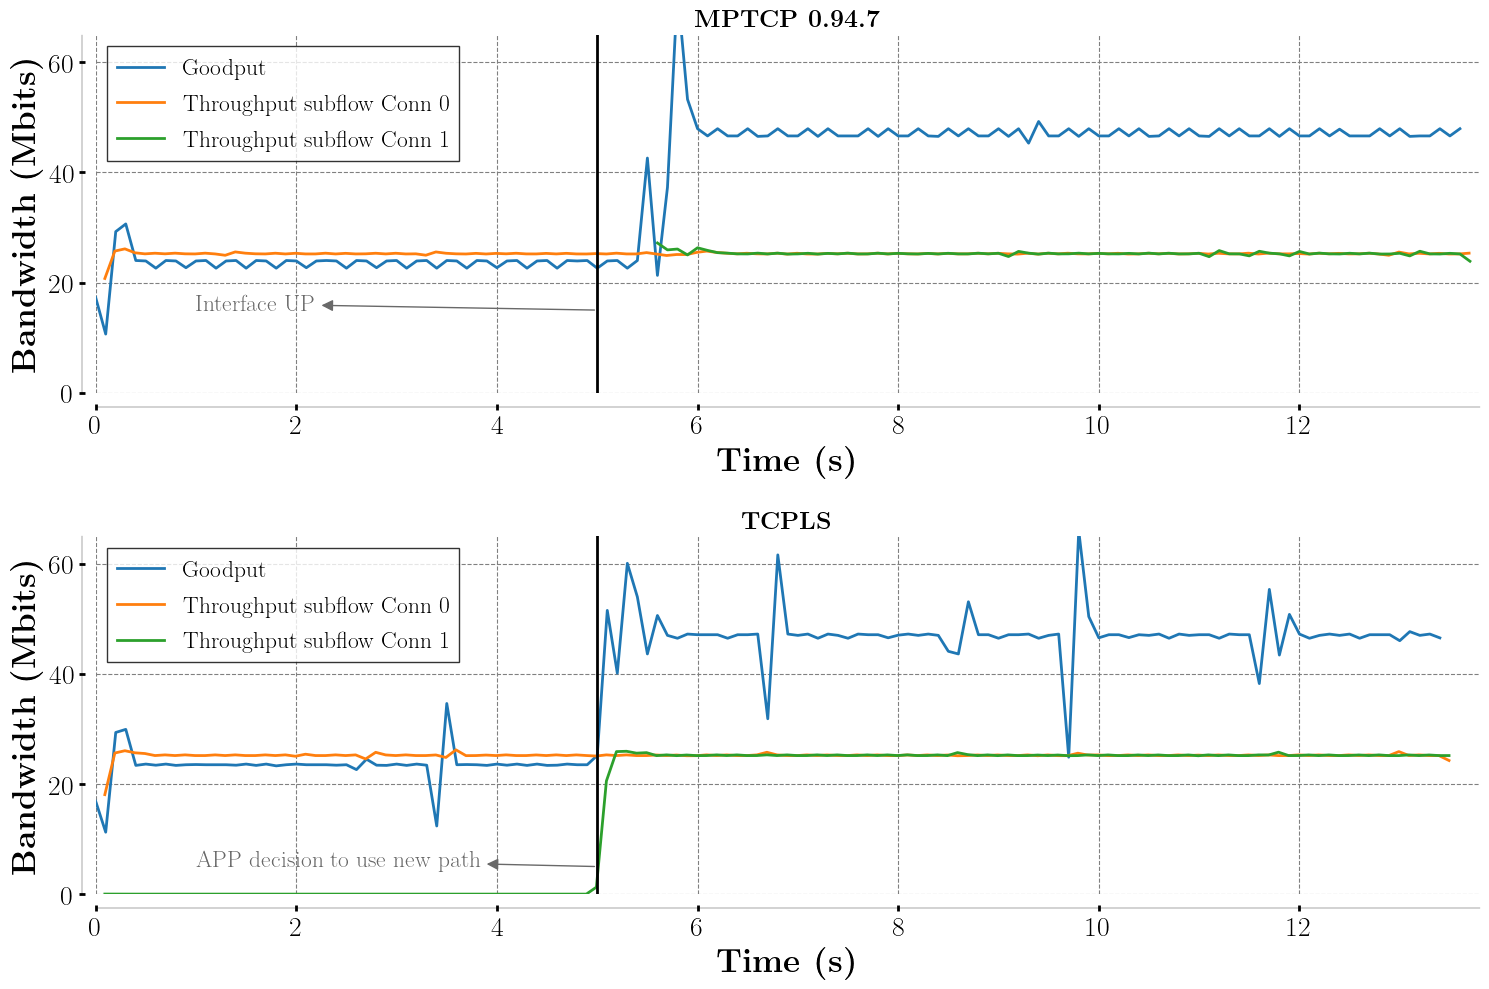
\includegraphics[width=.8\columnwidth]{figures/aggregate_1500bytes_records_dual.png}
  \caption{\tcpls path aggregation with 1500, bytes record size, compared to
    \tls over \mptcp with 16,384 bytes record size}
  \label{fig:aggregation_1500bytes_records}
\end{figure}

%\section{Artifacts description for AEC}
%
%As part of the artifacts released with this work, we release the TCPLS source 
%code, the scripts used for starting the experiments presented and 
%the scripts used to generate the figures of the paper.
%
%The source code contains 9k additional lines of C code we implemented on top of 
%\texttt{picotls} supporting the presented 
%features\footnote{\url{https://github.com/pluginized-protocols/picotcpls/}}.
%
%Figure \ref{fig:vegasCubic} can be reproduced by following a README on a 
%separate 
%branch\footnote{\url{https://github.com/pluginized-protocols/picotcpls/blob/tcpls/bpf-cc/t/ipmininet/readme_for_bpf_cc_test.md}}.

%Other figures presenting experiments results


\end{document}
